\documentclass[12pt]{article}

\usepackage[margin=0.5in, includefoot]{geometry}
\usepackage{setspace}
\usepackage{titlesec}
    \titleformat{\subsubsection}{\normalfont\normalsize\itshape}{\thesubsubsection}{1em}{}
\usepackage{hyperref}
\usepackage{xurl} % yay this works
    \hypersetup{
        colorlinks=true, 
        linkcolor=blue, % can comment this out if the blue figure faces is bothersome
        urlcolor=cyan
    }
    \renewcommand{\figureautorefname}{\textbf{Figure}} % decent fix but later should figure out how to make numbers bolded too
\usepackage{enumitem}
    \setlist[enumerate]{label=(\arabic*)}
\usepackage{amsmath}
\usepackage{amssymb} % for mathfrak font style
\usepackage{mathrsfs} % for mathscr font style
\usepackage{bm}
\usepackage{physics}
\usepackage{cancel}
\usepackage{xfrac}
\usepackage{array}
\usepackage{multicol}
\usepackage{float}
\usepackage[many]{tcolorbox}
    \definecolor{cellborder}{HTML}{CFCFCF}
    \definecolor{cellbackground}{HTML}{F7F7F7}
\usepackage{listings}
    \lstset{
        basicstyle=\scriptsize\ttfamily, % font style
        escapeinside={(*@}{@*)} % escape into LaTeX using (*@ and @*)
    }
\usepackage{subcaption}
\usepackage{wrapfig}
\usepackage{graphicx}
\usepackage{multirow}
\usepackage{csvsimple}
\usepackage[font=small]{caption}
\usepackage{xcolor} % for formatting purposes
\usepackage{lipsum} % for formatting purposes
% \usepackage[hang, flushmargin]{footmisc} % seeing if default setup is actually nice looking

\renewcommand{\thesubsection}{\arabic{subsection}}
\newcommand{\displayinline}[1]{\displaystyle#1\mathstrut}
\newcommand{\totder}[2][]{\frac{\mathrm{d}#1}{\mathrm{d}#2}} % needs amsmath package
\newcommand{\parder}[2][]{\frac{\mathrm{\partial#1}}{\mathrm{\partial#2}}} % needs amsmath package
\newcommand{\thetadot}{\dot{\theta}}
\newcommand{\thetaddot}{\ddot{\theta}}
\newcommand{\g}{\;\mathrm{g}}
\newcommand{\s}{\;\mathrm{s}}
\newcommand{\Hz}{\;\mathrm{Hz}}
\newcommand{\radian}{\;\mathrm{rad.}}
\renewcommand{\Re}{\mathfrak{Re}} % these are just cooler
\renewcommand{\Im}{\mathfrak{Im}}
\newcommand{\im}{\mathrm{i}}
\newcommand{\diff}[1]{\text{d}#1}
\newcommand{\R}{\mathbb{R}}

\newcommand{\wrt}{\textit{w.r.t.}\;}
\newcommand{\dragforce}{\vec{F}_d}
\newcommand{\forceofgravity}{\vec{F}_g}
\newcommand{\inversetanh}{\tanh^{-1}}


\newsavebox\foobox
\newlength{\foodim}
\newcommand{\slantbox}[2][0]{\mbox{%
        \sbox{\foobox}{#2}%
        \foodim=#1\wd\foobox
        \hskip \wd\foobox
        \hskip -0.5\foodim
        \pdfsave
        \pdfsetmatrix{1 0 #1 1}%
        \llap{\usebox{\foobox}}%
        \pdfrestore
        \hskip 0.5\foodim
}}
\def\Lagrangian{\slantbox[-0.2]{$\mathcal{L}$}} % ok wow nailed it (I think?)
\def\Fourier{\slantbox[-0.45]{$\mathscr{F}$}} % kinda legible yeah

%%%%%%%%%%%%%%%%%%
% begin document %
%%%%%%%%%%%%%%%%%%
\begin{document}
\setstretch{1.15}

\section*{Analytical Results on Hyperbolic Tangent and Neural Network Regression for Terminal Velocity}

\begin{quote}
    Jeff Lam, Jacob Volosik \\
    \textit{Department of Physics, Binghamton University} \\
    April 7\textsuperscript{th}, 2025
\end{quote}

\subsection*{Abstract}
An extensive study on the underlying trend of the motion of a free-falling object approaching terminal velocity was carried out,
including a thorough procedure on transforming position data into accurate velocity data as well as steps required to filter out any noise acquired during experimental runs.
As a side result, terminal velocity was shown to be proportional to the square-root of an object's mass,
yielding an experimental result of 15.424 for the collective coefficients of the drag force $D$ from a linear least-squares fitting result of $m=0.798\pm0.017$ as slope and $b=0.54\pm0.049$.
For the main result, a first principle derivation for the general solution of velocity for a free-falling diagram experiencing air resistance yielded $v=u\tanh(\dfrac{g}{u}t)$,
where $u$ represents the value of terminal velocity.
After transforming all available velocity data via $x=\dfrac{gt}{\norm{u}}$ and $y=\dfrac{v}{u}$,
a scatterplot of the available data hints at the underlying function $\tanh()$, but also reveals trouble for standard statistical regression techniques.
Motivated to use machine learning models instead, two approaches were thought out: gradient descent-guided polynomial fitting to conform with the Taylor expansion of $\tanh()$,
and general function fitting using neural network regression.
Ultimately, the former approach was deemed difficult to implement and latter approach yielded attractive results in showing that, with enough data, calculated velocity data on a free-falling object approaching terminal velocity indeed converges toward $\tanh()$ as the trend.

\noindent\rule{\linewidth}{0.5pt}

\begin{multicols}{2}

\subsection{Introduction}
In the typical classroom for introductory physics,
it is common to neglect air resistance in order to study the basics of kinematics.
This paper in comparison studies data gathered on the retarding effects of air resistance towards a free-falling object.
To this end, a theoretical framework surrounding the motion of a free falling object approaching terminal velocity must first be established.

\subsubsection{Free-body Diagram}
Air resistance is a direct consequence of Newton's Third Law of Motion, for when an object uses force to move through and displaces fluid (\textit{i.e.}, gas or liquid) the object experiences a (typically) equal and opposite force with respect to its motion.
This is commonly known as the \textit{drag force} $\dragforce$ in this scenario.
While the direction of $\dragforce$ may certainly be determined according to Newton's Third Law, the magnitude of the vector may depends on multiple factors.
In general, $\dragforce$ may be defined as the following equation which is known as the \textit{drag equation}:
$$\dragforce=\frac{1}{2}\rho\vec{v}^2C_dA$$
where $\rho$ represents the density of the fluid, $\vec{v}$ is the velocity of the moving object, $C_d$ is the drag coefficient, and $A$ is the cross-sectional area that a fluid region may ``see'' towards the incoming direction of the object [\hyperref[sec:1]{1}].

\textbf{Figure 1} illustrates the appropriate free-body diagram drawn for a free-falling object experiencing drag force due to air resistance.
The length of the vectors are emphasized to show that the two forces, the \textit{force of gravity} $\forceofgravity$ and drag force, are initially unequal.
According to the drag equation, with all other values being constant drag force increases with an object's speed proportionally squared.
An object is said to be at ``terminal velocity'' when $\dragforce$ grows to be equal to $\forceofgravity$, \textit{i.e.,}
$$\dragforce=\forceofgravity$$
It can be observed then that the free-body diagram shifts from obeying Newton's Second Law of Motion ($\sum\vec{F}=m\vec{a}$) to Newton's First Law of Motion ($\sum\vec{F}=0$),\
\textit{i.e.,} the object can be said to be in \textit{dynamic equilibrium}, and furthermore as a much more important implication, $\displaystyle{\totder[\vec{v}]{t}}=0$.

\subsubsection{(Differential) Equation of Motion}
From the drag equation, let $D$ represent all constants multiplied within the right-side of the equation, so $\dragforce=D\vec{v}^2$.
Using Newton's Second Law of Motion as described in the previous section,
a differential equation for its motion can be written as
$$m\totder[v]{t}=mg-Dv^2$$
where the vector notation for $\vec{v}$ has been dropped for convenience.

Using Newton's First Law of Motion as also described in the previous section,
let $u$ represent the speed of the free-falling object once terminal velocity has been achieved.
Then $\dragforce=\forceofgravity$ can be written as
$$mg=Du^2$$
From here, the equation can be used to derive two seperate relationships for individual analysis:
\begin{figure}[H]
    \centering
    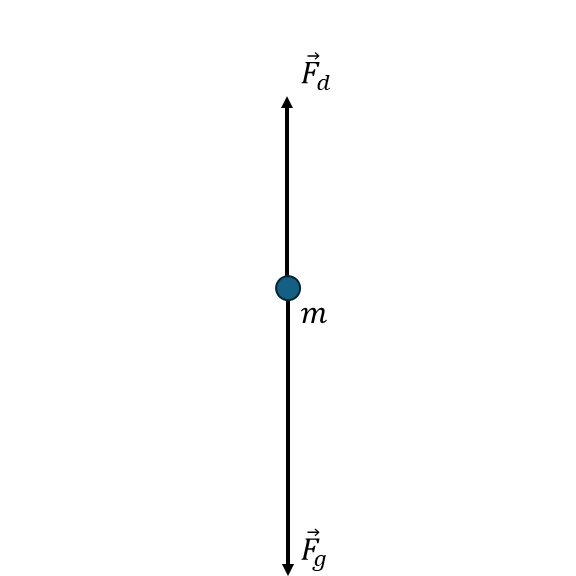
\includegraphics[width=0.98\linewidth]{figs/figure1.png}
    \caption{Schematic illustation of a free-falling object approaching terminal velocity.}
    \label{fig:1}
\end{figure}
% \begin{quote} % this is an option
    \begin{enumerate}[label=(\arabic*)]
        \item $u=\sqrt{\dfrac{mg}{D}}$ when used to solve for $u$;
        \item $D=\dfrac{mg}{u^2}$ when used to solve for $D$
    \end{enumerate}
% \end{quote}
The use of (1) has been shown in section \textit{3.4 Linear Least-squares Fitting} to show that terminal velocity $u$ is proportional to the square root of the object's mass, $\sqrt{m}$.
For this section, the results of (2) will be used to solve for the differential equation with respect to $v$.

\subsubsection{Solving for $v$}
Use the result $D=\dfrac{mg}{u^2}$ as a substituting value to get
$$m\totder[v]{t}=mg-\frac{mg}{u^2}v^2$$
where $m$ can be cancelled out on both sides to simplify and get
$$\totder[v]{t}=g-\frac{g}{u^2}v^2$$
To prepare in solving the differential equation via separation of variable,
the right-hand side of the equation can be rewritten as $\dfrac{g}{u^2}(u^2-v^2)$,
and dividing both sides of the equation with $(u^2-v^2)$ yields
$$\frac{1}{u^2-v^2}\totder[v]{t}=\frac{g}{u^2}$$
which can be integrated to solve for $v$ as the form
$$\int_{v_0=0}^v\frac{1}{u^2-\tilde{v}^2}\diff{\tilde{v}}=\int_{t_0=0}^t\frac{g}{u^2}\diff{\tilde{t}}$$
where the use of tilde \textsubscript{\Large\textasciitilde} represents dummy variable of integration. % this was so scuffed: https://tex.stackexchange.com/questions/9363/how-does-one-insert-a-backslash-or-a-tilde-into-latex

The general solution for the left-side integral of the equation can be found in \textbf{Appendix A: Full analytical solution for \bm{$\int\frac{1}{a^2-x^2}\diff{x}$}}.
For this paper, the solution of $\dfrac{1}{a}\inversetanh\qty(\dfrac{x}{a})$ was chosen out of all analyitcal solutions.
Then the differntial equation is solved as
$$\frac{1}{u}\inversetanh\qty(\frac{v}{u})=\frac{g}{u^2}t$$
After a cancelation of a $u$ in both side's denominators, the general solution for $v$ is solved for and obtained by taking $\tanh()$ on both sides:
$$v=u\tanh\qty(\frac{g}{u}t)$$
A remarkable result with this derivation is the fact that as a direct consequence of performing $\tanh\big(\inversetanh()\big)$,
the ratio $\dfrac{v}{u}$ in this form is bounded by $\pm1$, \textit{i.e.}, $-1\leq\dfrac{v}{u}\leq1$ due to the domain restriction,
but since any graph of this going from positive to negative and \textit{vice versa} indicates a direction change,
it is much more appropriate to state that $\dfrac{v}{u}$ is bounded by $0$ and $1$.
This means that the mathematical derivation for this general solution is quite grounded to the physical world,
as it indeed reflects correctly on our assumption that $\dragforce=\forceofgravity$ when terminal velocity is reached.
\begin{figure}[H]
    \centering
    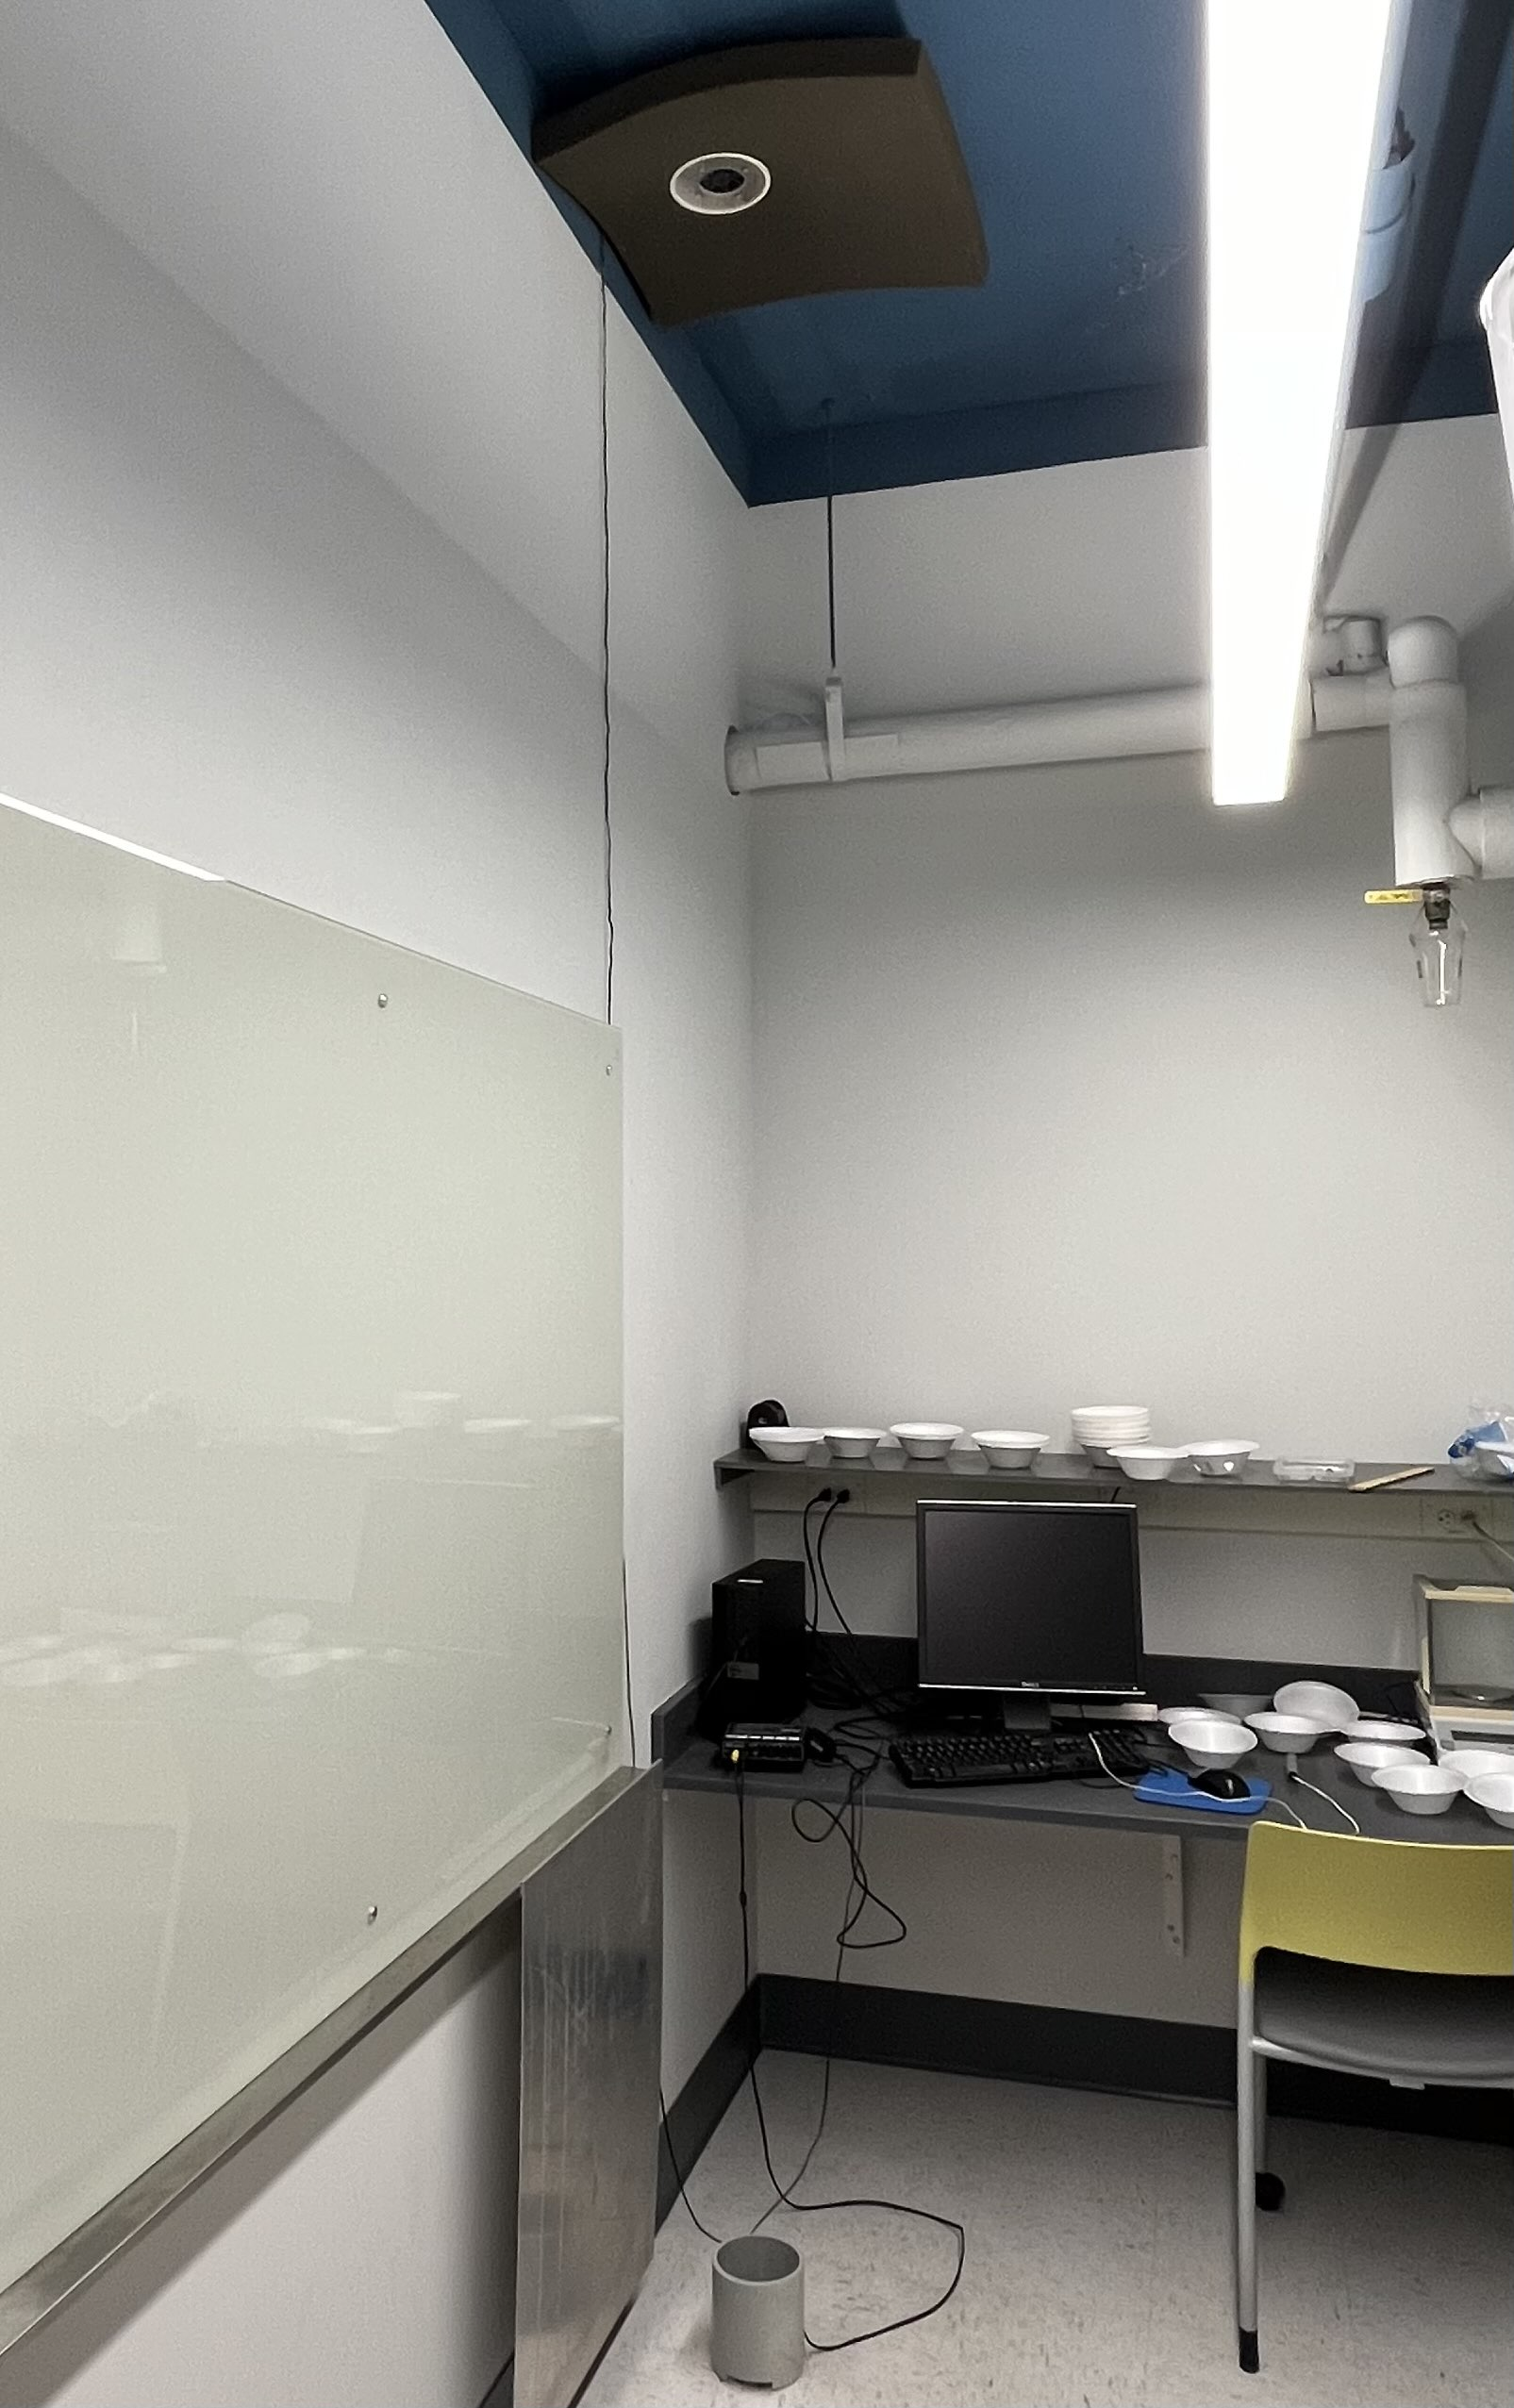
\includegraphics[width=0.98\linewidth]{figs/figure2.jpg}
    \caption{Photograph of the experimental setup in the lab.}
    \label{fig:2}
\end{figure}
\subsection{Methods}
\subsubsection{Experimental Setup}
\textbf{Figure 2} helps visualize the experimental setup for measuring the position of a free-falling object approaching terminal velocity.
The choice of object for free-fall was a styrofoam bowl for its lightweight nature as well as large cross-sectional area to maximize drag (all as compared to, say, a ball).
In order to later in this paper perform linear least-squares fitting to show the proportionality between $u$ and $\sqrt{m}$,
four additional styrofoam bowls were selected and had different amounts of washers taped at each their inner center,
varying in weight such that the styrofoam bowls successively increase in mass.
All together, including the styrofoam bowl without washers, five different styrofoam bowls were respectively weighed in as 2.978g, 8.029g, 9.397g, 11.1017g, and 12.169g using a precision scale.

At the top of the lab ceiling is a fan attached such that it continuously creates positive air pressure below, allowing a styrofoam bowl to be suspended until it is turned off.
Right directly below the position of the ceiling fan at floor of the lab is a cylindrical tube matching the divot of the bowl in width in order to ``catch'' it after it lands.
The height between the cylindrical tube and ceiling fan was approximately measured to be 3.5m.
Within the cylindrical tube is a motion sensor calibrated and set at the speed of sound value (approximately $331\mathrm{m/s}$ [\hyperref[sec:2]{2}]) to track the position of the styrofoam bowl as it falls.
PASCO Capstone was used as the software during data gathering, with the sampling rate set at 20 Hz.
All data gathered were then exported as a \texttt{.csv} file and overall compliled together into a master \texttt{.xlsx} (Microsoft Excel) file for later data manipulation in Python.

\subsubsection{Experimental Procedure}
All styrofoam bowls had 30 trials saved to conform with the statistics fact that a sample size of at least 30 allows a distribution to be approximately Gaussian [\hyperref[sec:3]{3}].
Unintentionally, this paper has specifically gathered 70 trials for the bowl with mass 8.029g.
For each trial, the chosen styrofoam bowl was suspended at the fan before data recording began.
Once data recording started, the fan was immediately turned off to allow the styrofoam bowl to start free-falling.

It is at this point that multiple outcomes may occur, but essentially two are boiled down and are described:
(1) the styrofoam bowl falls straight down and is caught nearly perfectly by the cylindrical tube;
or (2) the styrofoam bowl either drifts around during free fall and/or bounces off the cylindrical tube if it does not land perfectly.
For the case of (1), the data was certain to be normal and free of \textit{noise}, unlike the case with (2),
in which any deviation described would cause the motion sensor to inaccurately capture the position of the bowl as unusually higher than it normally should be.

It is suprisingly rare to capture data where the styrofoam bowl falls perfectly onto the cylindrical tube within a trial,
so some data gathered in this paper can be seen to have ``kinks'' in a few of its position points when graphed--- the noise manifesting in the data is dubbed by this paper as \textit{turbulence}.
For the case when the bowl's deviation completely messes up the recording,
such as the bowl not being caught by the cylindrical tube and therefore causing the motion sensor to ``spike'' its position reading back to 3.5m,
the data was immediately and completely discarded before re-running the trial.
This procedure was repeated for each styrofoam bowl until at least 30 trials of data ranging in quality from perfect at best to semi-usable at worse were gathered.

\subsection{Data Analysis}
\subsubsection{Calculating velocity data}
In the field of numerical methods, there exists a few methods in regard to calculating the ``derivative'' of a given array of data.
Namely, the forward difference, backward difference, and central difference approximation methods which are each some sort of analogue to the formal definition of a derivative:
$$\totder[]{x}f(x)=\lim_{h\to0}\frac{f(x+h)-f(x)}{h}$$
where $h$ is the $x$-related spacing of the dataset.
In general, the central difference approximation is considered as a more accurate approximation to a dataset's derivative than either of its counterparts.

PASCO Capstone software automatically calculates the velocity of a tracked object during recording,
but due to uncertaincy in the method employed, only raw data of the categories time and position were exported for each trials.
With Python being used instead, a standard numerical module \texttt{numpy} allows reliable calculation of velocity data given an array of position data via \texttt{numpy.gradient()}, which uses a combination of the numerical methods mentioned previously---
employing central difference to approximiate the derivative among most of the data and only using forward/backward difference approximations on the end points
(if it is of any interests as well, this means that only the endpoints suffer from an error of $\mathcal{O}(h)$ while the rest of the data enjoys only having an error of $\mathcal{O}(h^2)$).
This has another major benefit: the size of the derivative array also matches the size of the input array due to this method [\hyperref[sec:4]{4}].
This sameness in array size makes filtering noisy data from semi-perfect trial runs as shown in the next section much easier.

\subsubsection{Filtering Turbulence}
\textbf{Figure 3} showcases plots of position vs.\;time and calculated velocity vs.\;time graphs for datasets from a perfect and turbulent trial run.
As it can be seen, the absence of any kinks within the position data for a clean dataset allows normal values of calculated velocity data to appear in (b).
Meanwhile, for the case of kinks appearing due to an imperfect trial run, the resulting calculated velocity data contains outliers way off of normal parameters as a result.
Herein lies the main issue regarding data analysis in this paper: filtering the turbulent data points across all 190 trial runs.

This paper employs the following method to remove the kinks within the datasets:
(1) a convolution of the velocity dataset using a kernel array of $[0,\;-1,\;1]$ for edge detecting as the first transformation;
then (2) calculating respective $Z$-scores for each convolution signal to allow the filtering of outliers that fall outside a specified critical $Z$-score value $Z_\text{critical}$.
\begin{figure}[H]
    \centering
    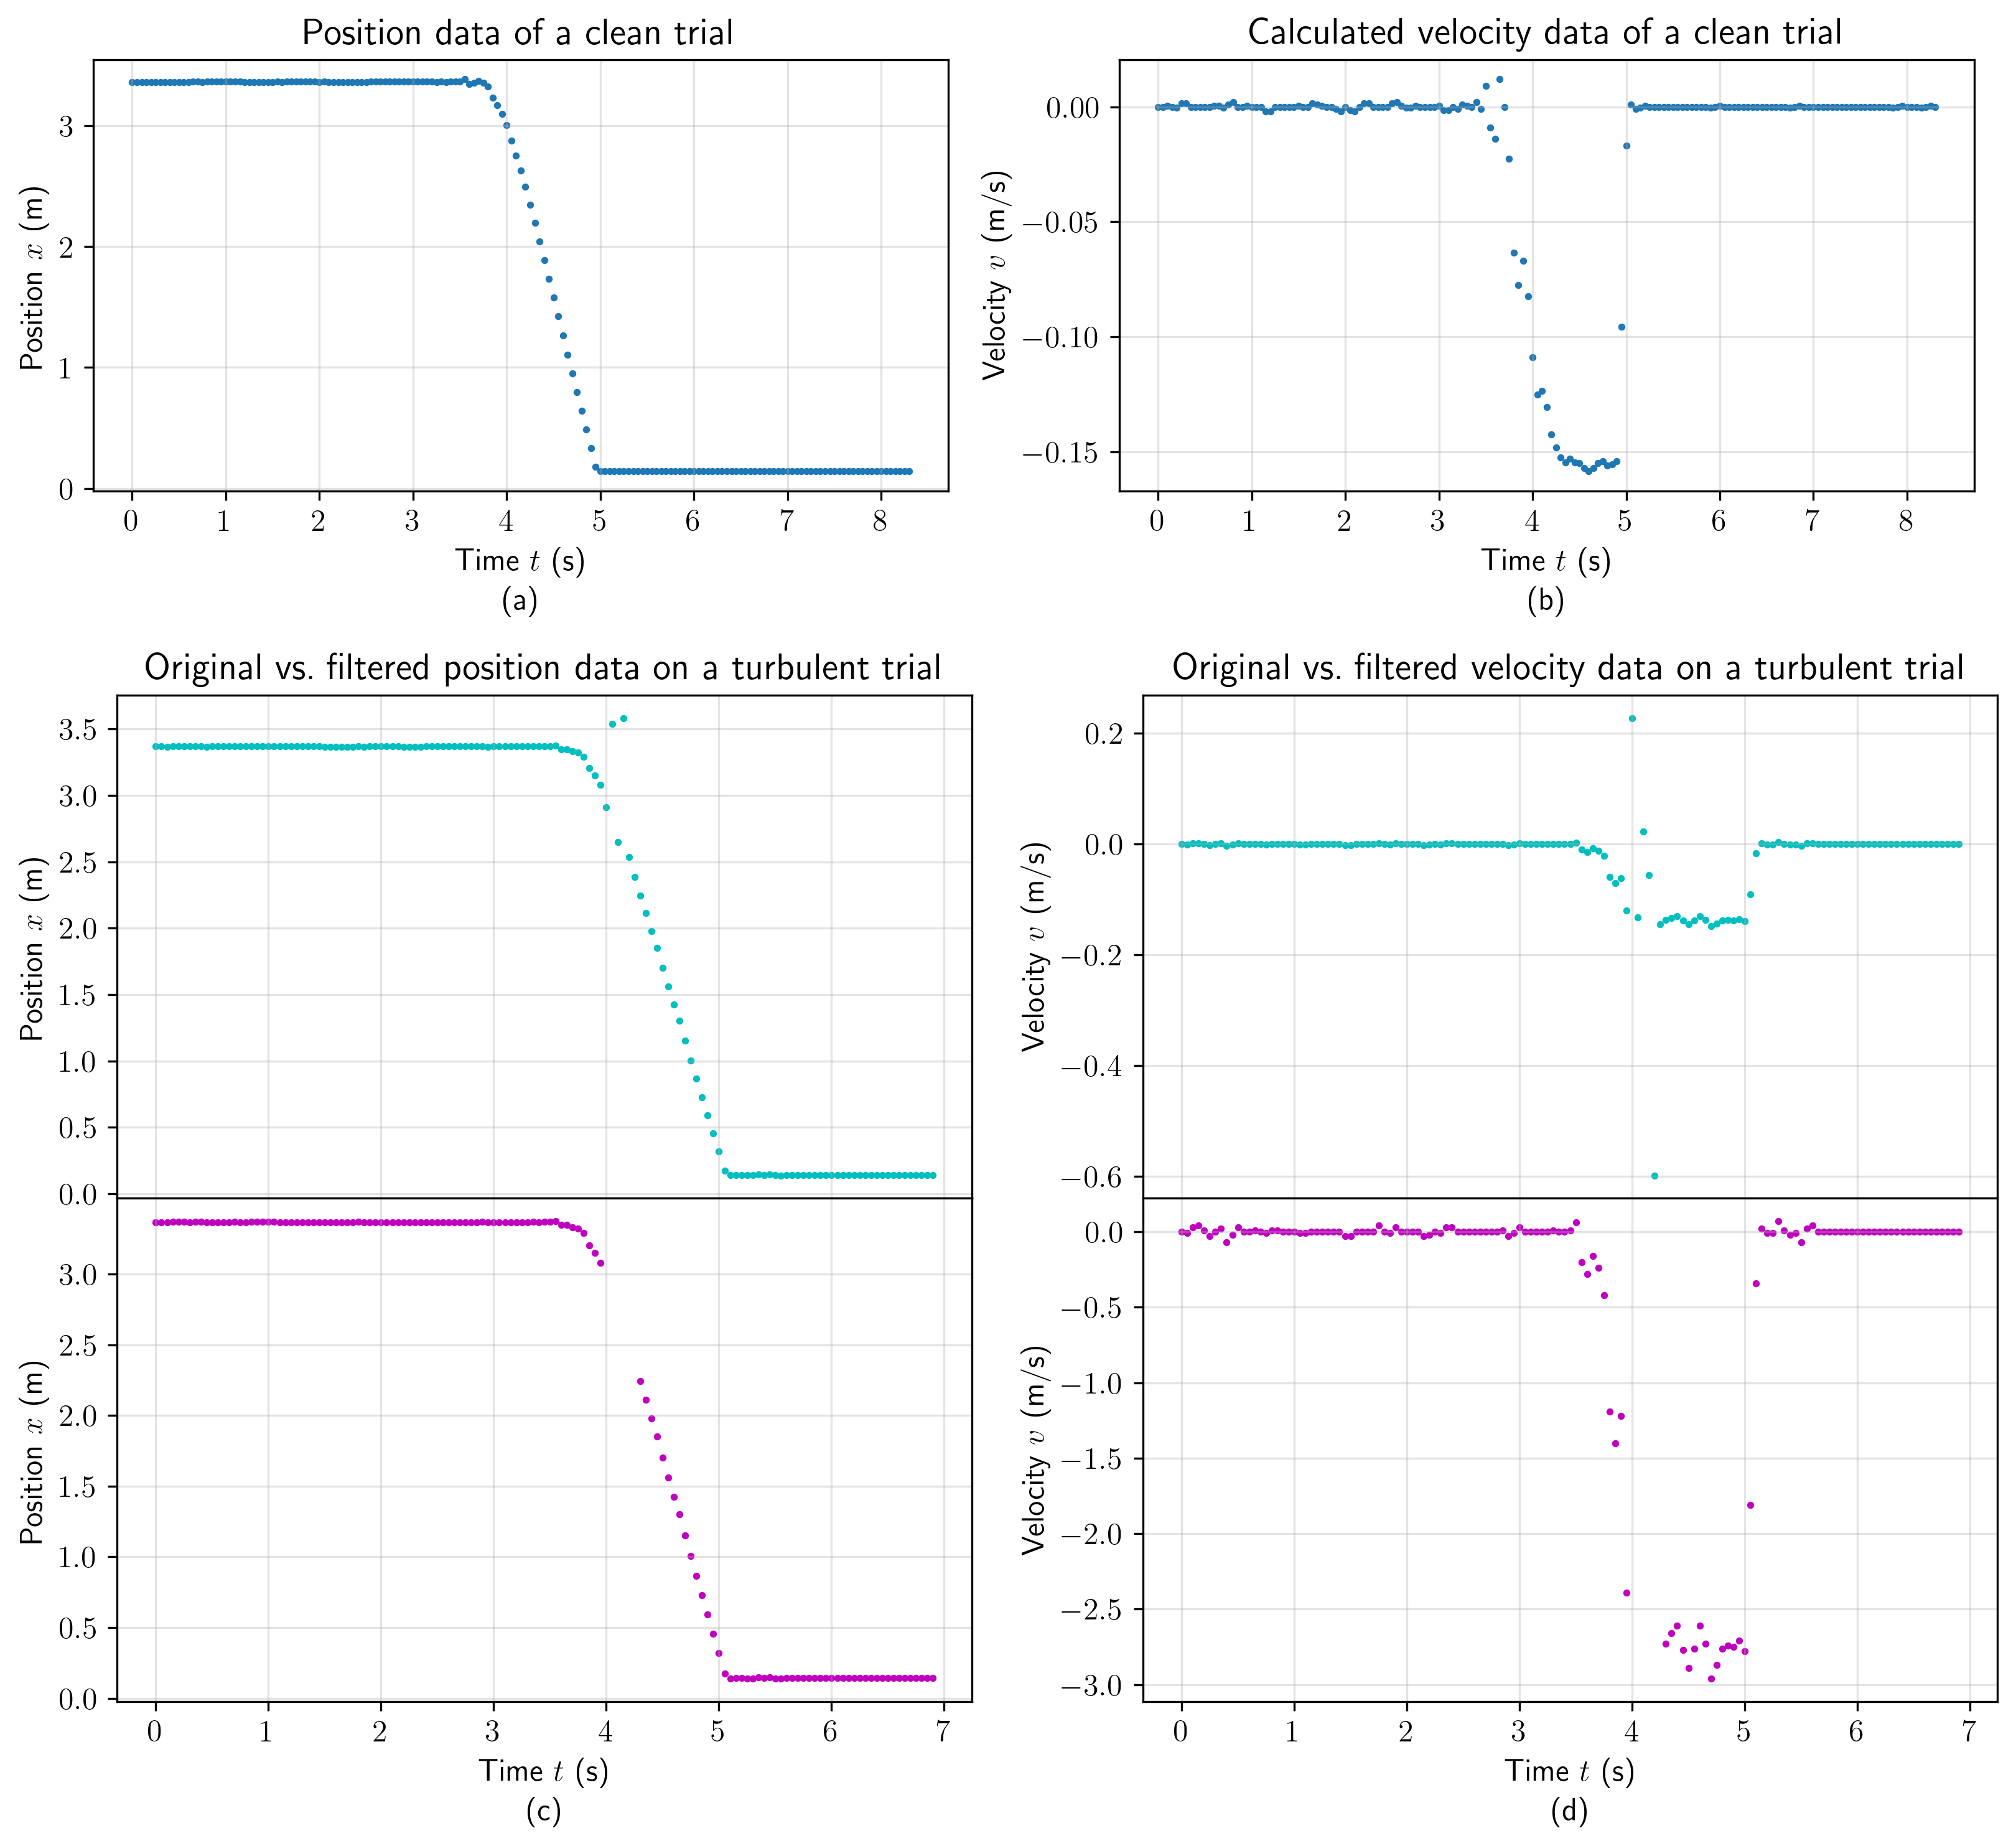
\includegraphics[width=0.98\linewidth]{figs/figure3.png}
    \caption{
        Various position vs.\;time and calculated velocity vs.\;time graphs of two sample datasets.
        (a) \& (b) represents the case of working with a ``clean'' dataset,
        while (c) \& (d) represents the additional work needed to remove kinks within a turbulent dataset,
        where the cyan represents the original data from the trial while magenta represents the same data after sufficient filtering.
        A threshold of 1 for the $Z$-score was used to filter out the outliers for this case.
    }
    \label{fig:3}
\end{figure}
\noindent
This $Z_\text{critical}$ is dubbed by this paper as the \textit{threshold} for filtering turbulence.
This duo of transformation ensures two actions:
(1) preventing any loss of data from a perfect trial, for all $Z$-scores calculated in this scenario should be 0;
and (2); properly filter out the calculated velocity outliers from semi-usable datasets, as shown exemplarily in \textbf{Figure 3d}.
It is worth noting that given the analysis method outlined by this paper, it is \textit{not possible to simply remove the kinks from turbulent data outright},
for \texttt{numpy.gradient()} assumes the array of data to be all evenly spaced in $h$ value and neither is there a simply transformation to fix the dataset after removing the kinks
(\textit{e.g.,} shifting the dataset to ``close the gap'' left by the kinks would then create a jump discontinuity within the position data and \textit{etc}.)
The position kinks removed in the magenta scatterplot in \textbf{Figure 3c} was removed as a consequence of the filtering process (for all calculations and transformations are saved next to the original data).

\subsubsection{Terminal Velocity}
Armed with a functional programming procedure to filter out the majority of kinks,
all datasets were subject to a $Z$-score filtering of a threshold of 0.5 (\textit{i.e.}, $Z_\text{critical}$=0.5) before obtaining a terminal velocity value for each run as the minimum of the calculated velocity data.
This threshold value was determined via trial-and-error, for a threshold value too large would not filter out enough kinks amongst the conglomerate dataset and a threshold value too small would start ruining the terminal velocity value obtained for some runs
(code for \textit{saving} the same plots seen in \textbf{Figure 3} may be viewed in in \textbf{Appendix C: Full analysis across all data}).
All code ran for the data can be viewed in \textbf{Appendix C}.

\subsubsection{Linear Least-squares Fitting}
Using the relationship between $u$ and $m$ that was derived in section \textit{1.2 (Differential) Equation of Motion},
factoring out $g$ and $D$ as constants under the square-root implies the following proportionality:
$$u=\sqrt{\frac{g}{D}}\sqrt{m}\;\longrightarrow\;u\propto\sqrt{m}$$
Which also implies that a linear least-squares regression model is \textit{only appropriate} for the proportionality between terminal velocity and the square-root of mass.
It is of interest of this paper then to also view the \textit{residuals} of a linear least-squares fitting $\varepsilon$ (\textit{i.e.}, $\hat{y}-y$) to determine the appropriateness of the model.

\textbf{Figure 4} shows the linear least-squares fitting for all terminal velocity values gathered vs.\;$m$ and $\sqrt{m}$ along with their respective residual plots.
Surprisingly, the coefficient of determination $R^2$ for the case of not transforming $m$ is still relatively high, with a value of approximately 0.907.
\begin{figure}[H]
    \centering
    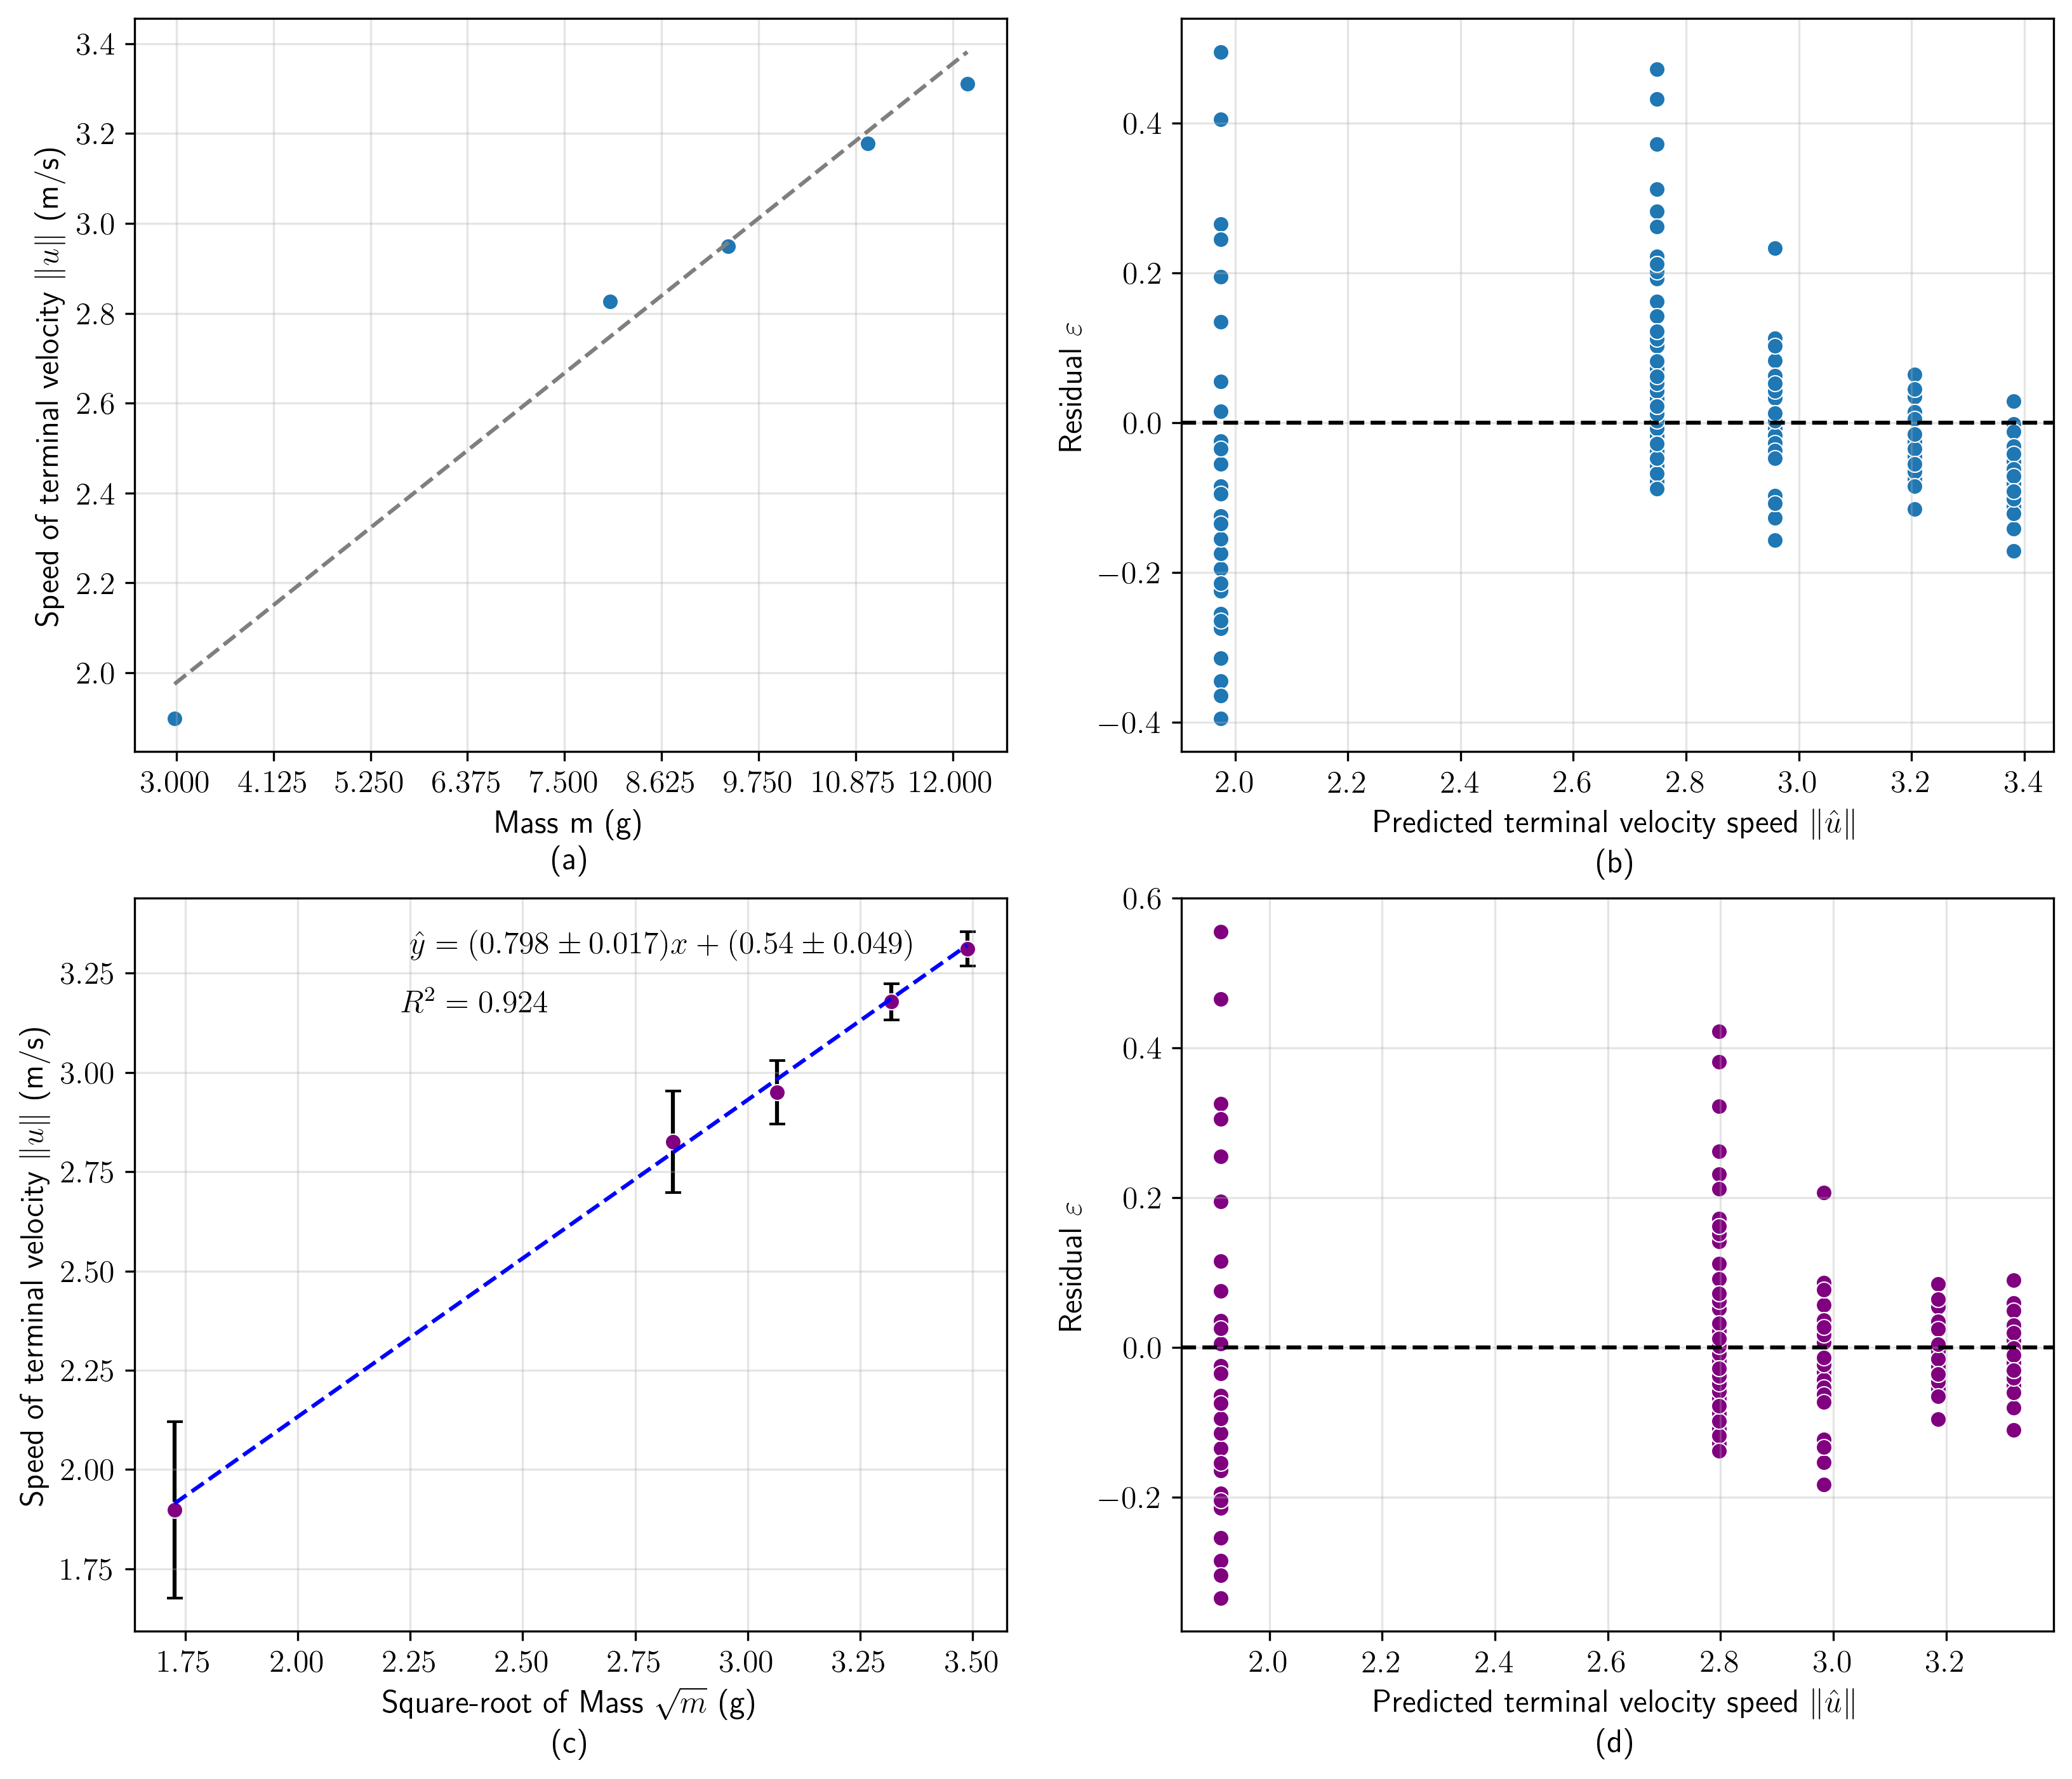
\includegraphics[width=0.98\linewidth]{figs/figure4.png}
    \caption{
        Respective linear least-squares fitting for the case when $m$ is untransformed and when it is $\sqrt{m}$.
        The predictive parameters and $R^2$ value for (a), for it is not included in graph,
        was found to be $m=0.1530\pm0.004$, $b=1.5191\pm0.032$, and 0.907, respectively,
        where $\pm$ values represents uncertainties reported in the form of standard deviation.
        Error bars represent standard deviation in dependent values as uncertainties.
    }
    \label{fig:4}
\end{figure}
\noindent
However, it is of this paper's belief that if more data were gathered across more mass values,
the scatterplot of the terminal velocity data should start to follow more of a \textit{square-root trend}, which would be a clear indication of linear least-square fitting being an unfit model.
In fact, it can be seen that by just transforming mass to $\sqrt{m}$, the data points begin shifting closer towards the line of best fit.
The residual plots also reflects these indications, for the residual clusters shown for $m$ alone follows a distinct pattern,
meanwhile the residual clusters for $\sqrt{m}$ are shifted more towards the $\varepsilon=0$ line.

Moreover, the slope of the linear trendline may represent the constant values factor out of the square-root,
$\sqrt{\dfrac{g}{D}}$, and so $D$ may be experimentally determined. Using $9.81\mathrm{m/s^2}$ as the constant value for $g$,
$D$ according to this experiment was calculated to be 15.424 in value.

\subsection{Advanced Regression Techniques}
\subsubsection{Setup for $y=\tanh(x)$}
With the other result derived in section \textit{1.3 Solving for $v$}---
the general solution for $v$ of a free-falling object experiencing air resistance $v=u\tanh(\dfrac{g}{u}t)$---
it may also be of interest to verify if this trend can be found across all calculated velocity data.
Thanks to the work done to produce \textbf{Figure 4},
every trial run has an acceptable terminal velocity value associated
(where each values were verified to be acceptable by plotting tangent lines to the position data as mentioned in section \textit{3.3 Terminal Velocity}).

Let $x$ and $y$ be the transformations $\dfrac{gt}{u}$ and $\dfrac{v}{u}$, respectively.
These transformations are essentially \textit{normalization} of the velocity data, and should allow the plot to take the form $y=\tanh(x)$.
Additionally, since $v$ and $u$ are calculated to be negative, one must be careful when considering when to use absolute value of either or or not,
lest unintentionally flipping the perspective data over the $x$- and/or $y$- axes.
Since $v$ and $u$ are negative quantities, the ratio of the two becomes positive, meanwhile $t$ data gathered are always positive,
so $\norm{u}$ should be used to transform $x$ data, \textit{i.e.}, $x=\dfrac{gt}{\norm{u}}$.

\textbf{Figure 5} showcases all available (and appropriate) data transformed and plotted.
To prepare for considering advanced regressional techniques--- \textit{gradient descent-guided polynomial fitting} and \textit{neural network regression}---
efforts to transform as many velocity data were made while still removing any outliers as a result of kinks.
To this end, velocity datasets were transformed with a threshold value of 1 before following the transformation process as written in the captions.
Amongst the five groups of datasets with respect to mass, all except the trial runs for the styrofoam bowl of weight 2.978g had reasonable $x$ data transformations---
2.978g trial runs not only had exceeding large $x$ data transformations
\begin{figure}[H]
    \centering
    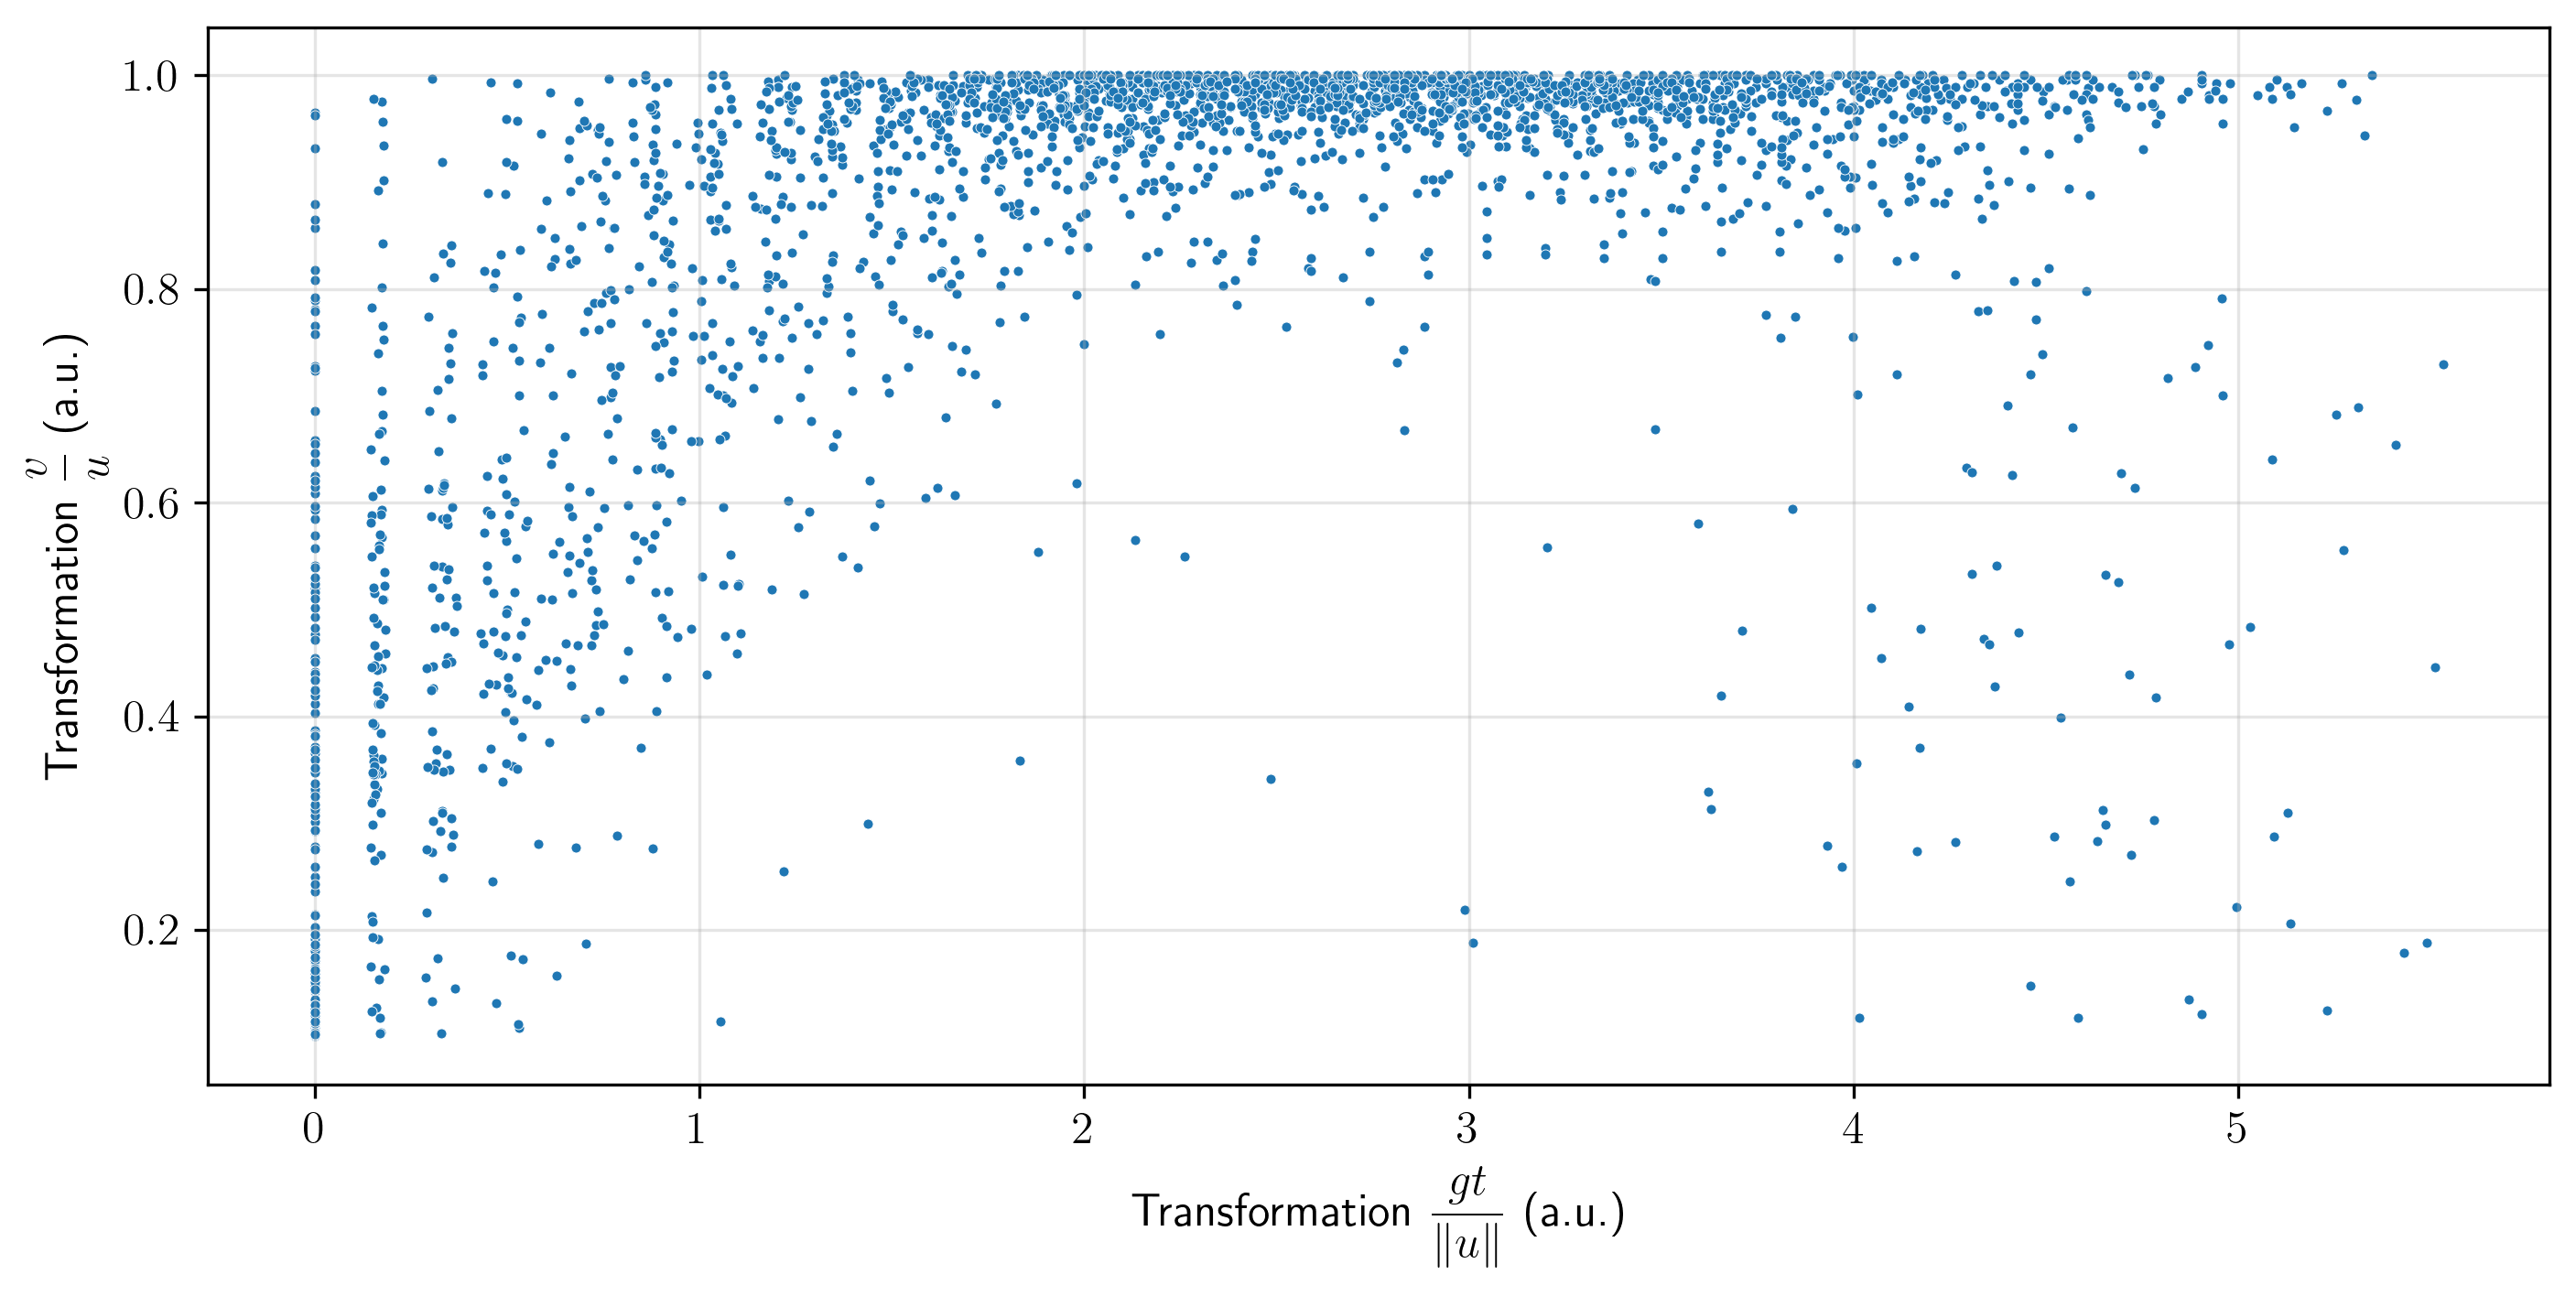
\includegraphics[width=0.98\linewidth]{figs/figure5.png}
    \caption{
        Plot of all transformed velocity data gathered across the trials ran for styrofoam bowls 8.029g, 9.397g, 11.1017g, and 12.169g.
        Datasets were first filtered with a threshold value of 1, transformed as outlined in section \textit{Setup for $y=\tanh(x)$},
        then further filtered to keep the data values where $0.1\leq\dfrac{v}{u}\leq1$. 
        Before conglomerating, each trial data had their $x$ data shifted to 0 using the first valid value filtered.
        Total size of the dataset collection yielded 2760 values.
    }
    \label{fig:5}
\end{figure}
\noindent
(of values between 0--14 as compared to what is shown in \textbf{Figure 5}),
but many trial-and-error with the threshold values yielded insufficiently cleaned data.
Therefore, the dataset was excluded from this conglomeration.

Regardless, it can be vaguely seen that the transformed velocity data follows a $\tanh()$ graph,
but despite employing the functional programming procedure as described previously here there still seems to exists quite some noise.
In order to verify that these data points follow the $\tanh()$ trend, one may be interesting in attempting to fit a curve through regression.
However, due to the literal ``scatter'' nature of the datapoints, not every datapoint is guaranteed to have a mean and standard deviation given some singular points may be seen on the plot (\textit{e.g.}, observe the right-most farthest point).
In this scenario, where there exists a large amount of data but no error bars are provided,
the next approach would be to trust every data point equally in an attempt to, in a sense, \textit{force} a regression line to form.
This is the basis and motivation behind \textit{gradient descent} and \textit{neural networks}.

\subsubsection{Attempts for Gradient Descent-guided Polynomial Fitting}
Since it is known that the trend in theory should follow the trend of $\tanh()$,
a natural appproach may be to choose \textit{polynomial fitting} on the data set.
Although difficult, the Taylor series expansion for $\tanh()$ can be determined,
which the full derivation can be found in \textbf{Appendix B: Taylor series expansion for hyperbolic tangent}. % weird bug?
Since $\tanh()$ is continuous unlike its normal trigonometric counterpart $\tanh()$,
the Taylor series expansion of function likely represents the function exactly similar in proof to $sin()$, $\cos()$, \textit{etc}.

One may infer then that \textit{comparing} the coefficient values for a polynomial fitting on the transformed velocity data to that of the coefficient terms of the Taylor expansion of $\tanh()$ would be a promising approach.
However, there is a direct conflict between this approach and gradient descent-guided polynomial fitting.
\textbf{Figure 6} shows the Taylor expansion around $x=0$ for $\tanh()$.
As it may be seen, higher order polynomial series does start to converge to the general function,
but nowhere near the range of values matching the scatterplot in \textbf{Figure 5} (\textit{i.e.}, convergent behaviour up to $x=5$).
Furthermore, the polynomial degree is already quite high---
using gradient descent to minimize the loss function of a polynomial becomes increasingly difficult the higher order the polynomial function becomes,
and makes it more susceptible to \textit{overfitting}.
Due to these limitation, while this non-linear regression approach seemed plausable,
this paper ultimately moved on to instead do \textit{general functions fitting} using neural networks and deep learning.

\subsubsection{Neural Network Regression}
Gradient descent as one of the fundamentals for machine learning is heavily built upon for deep learning---
\begin{figure}[H]
    \centering
    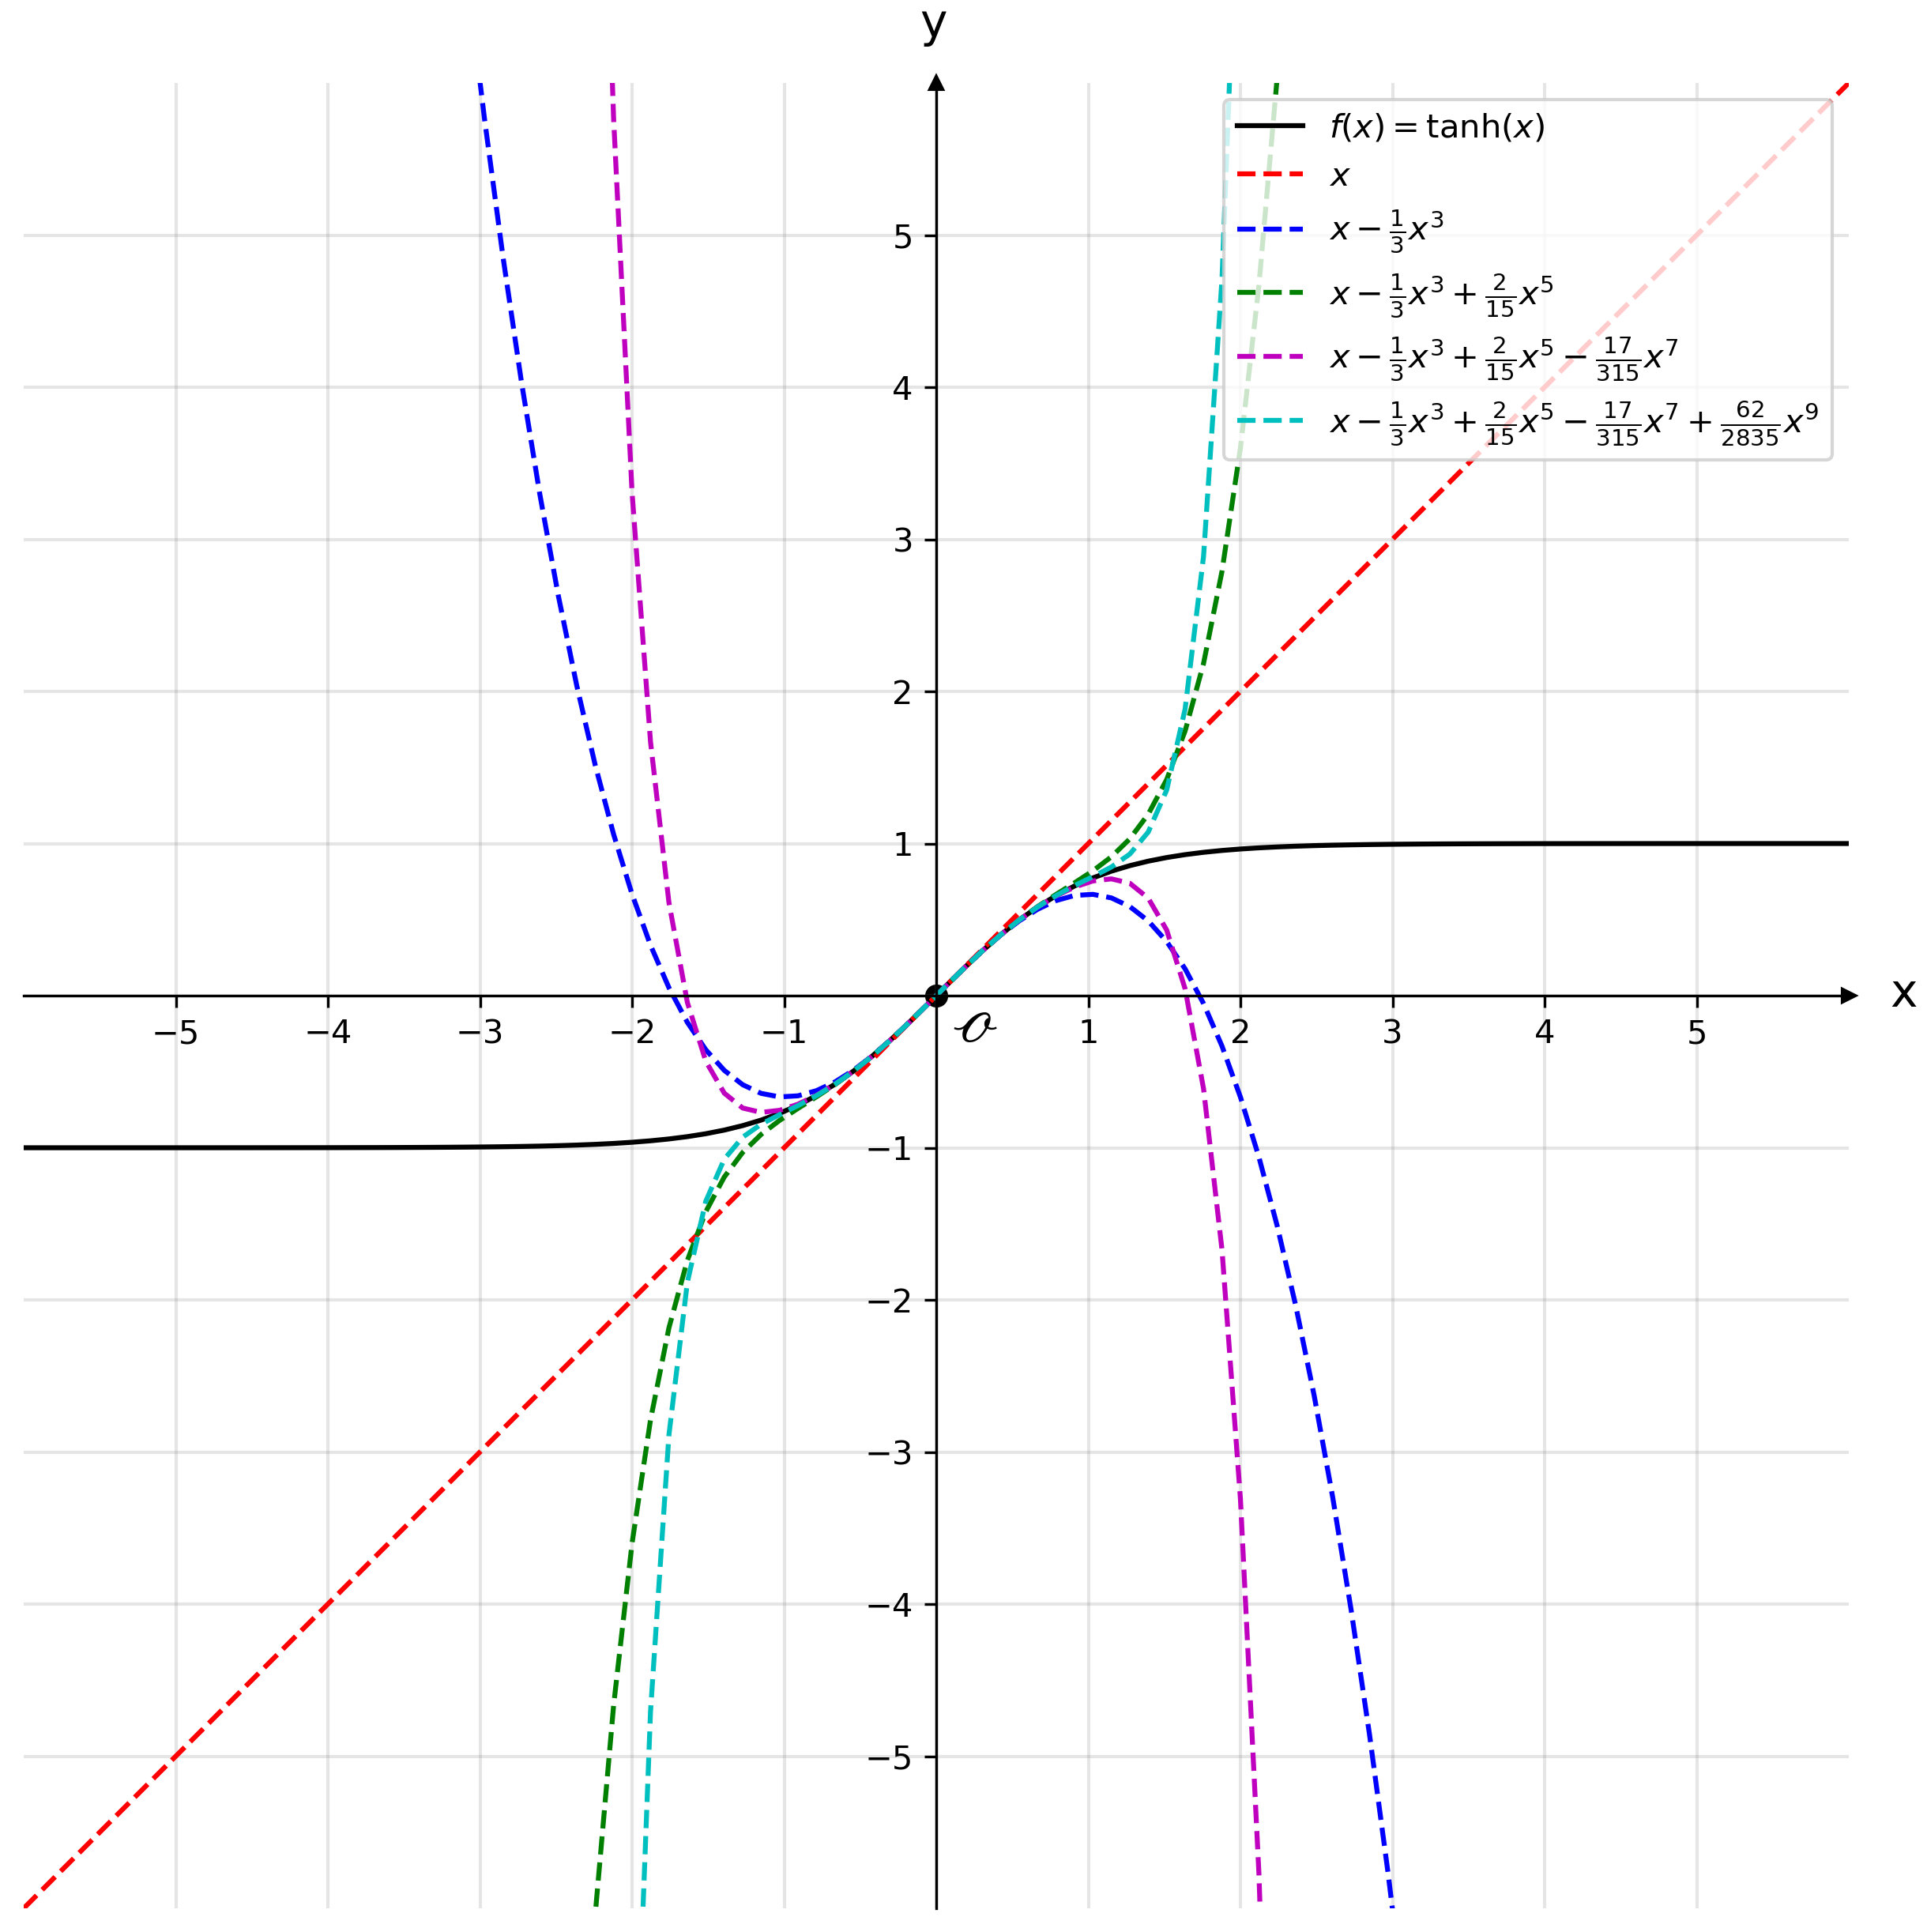
\includegraphics[width=0.98\linewidth]{figs/figure6.png}
    \caption{
        Taylor series expansion of $\tanh()$ at $x=0$ up to the 9th order. [\hyperref[sec:5]{5}]
    }
    \label{fig:6}
\end{figure}
\noindent
the process of creating \textit{neural networks} using nonlinear activation functions as hidden layers.
The use of nonlinear activation functions and line fits in a network-like manner essentially allows a machine to fit a general function trend in an efficient manner (since nonlinear functions allow ``shaping'' to the curve and line fits are computationally fast to perform).
Once a model is prepared, it is ready to ``train'' on data (without first setting aside some percentage of the data for validation in order to prevent overfitting) under a loss function of choice.
When a sufficiently low error rate has been achieved, the model is ready to predict input data as the general function trend.
Deep learning has many application for its powerful predictive purposes, however for this paper it shall be used for neural network regression.

Deep learning was carried out using the \texttt{pytorch} library in Python,
which is arguably considered as the industry standard coding library for deep learning,
but only by extension; a wrapper for the module called \texttt{fastai} was actually used to do all steps mentioned previously.
Additional parameters set for the deep learning processs:
\begin{enumerate}[label=(\arabic*)]
    \item CUDA was enabled for rapid training time;
    \item a valid percentage of 20\% was set aside from the total dataset;
    \item mini-batch gradient descent was peformed, using a batch size of 1380;
    \item root-mean square error was chosen as the loss function to minimize;
    \item a starting learning rate of 0.1 was chosen after plotting calling a learning rate finder method;
    \item 100 epochs were ran over the datasets.
\end{enumerate}
After training, a minimal loss value of 0.140943 was achieved.
\begin{figure}[H]
    \centering
    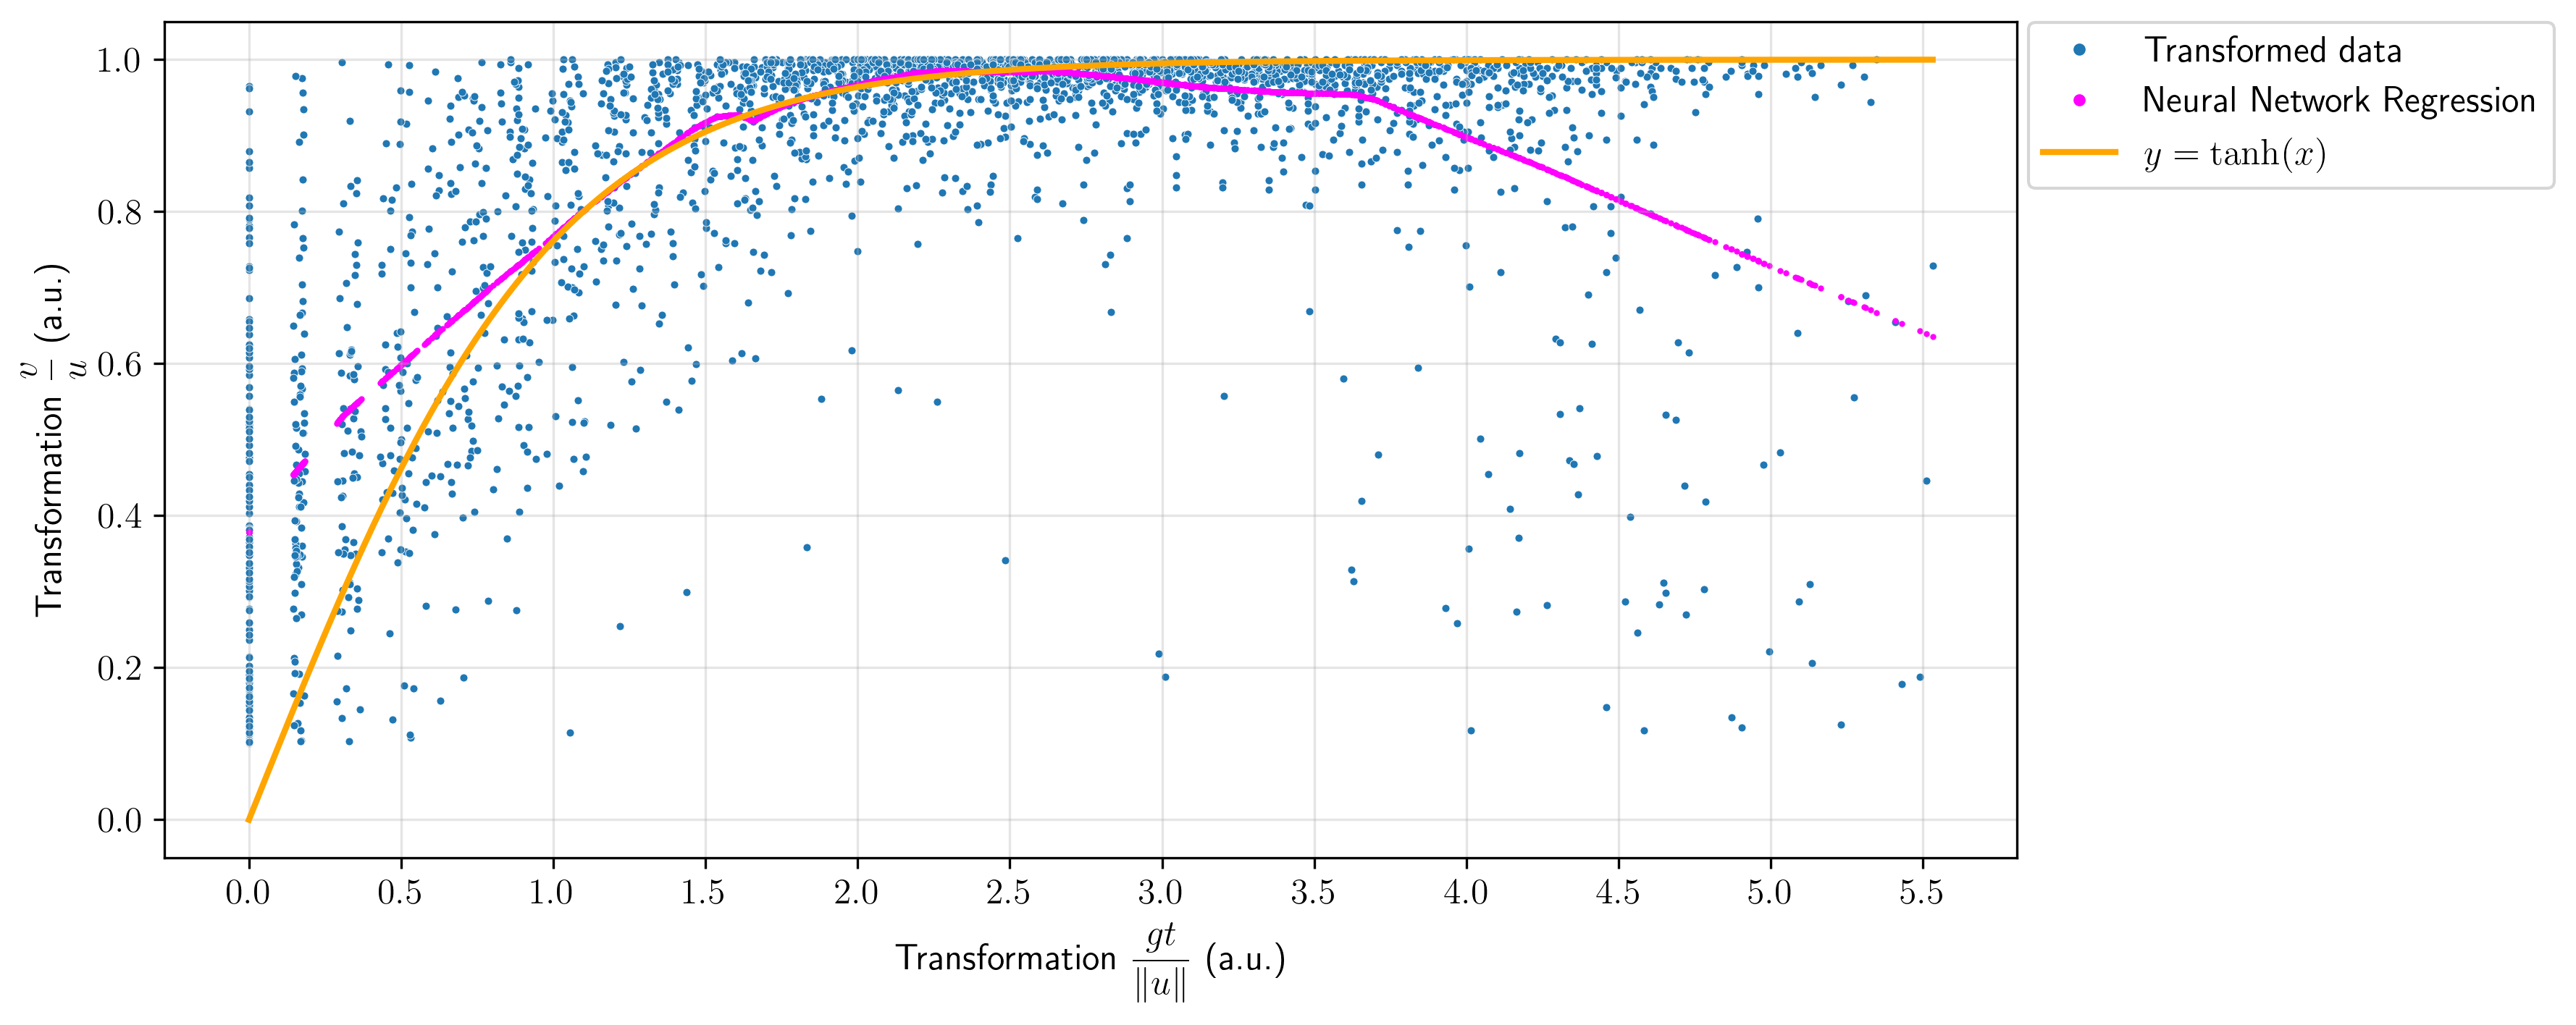
\includegraphics[width=0.98\linewidth]{figs/figure7.png}
    \caption{
        Results of the neural network regression on the total transformed velocity dataset.
        The underlying function, $y=\tanh(x)$, is also plotted for comparison.
    }
    \label{fig:7}
\end{figure}
\noindent
\textbf{Figure 7} shows the final results of the neural network regression.
As it can be seen, the regression model not only was successfully ploted, but also shows some convergent regions to the underlying function.
At the start of the regression, it overestimates a bit, which is expected as many transformation data corresponding to 0 was filtered out,
and towards the end of the plot it starts underestimating, which can clearly be attributed to the noisy region below the main datapoint cluster.
Overall though, it is of this paper's opinion that the neural network regression has done a decent job to show that velocity of a free-falling object approaching terminal velocity follows a $\tanh()$ trend
(\textit{i.e.,} it is enough to just \textit{qualitatively} assess the model rather than quantitatively interpret any error and such).

\end{multicols}
\newpage

\subsection*{References}
\begin{enumerate}[label={[\arabic*]}]
    \item \label{sec:1} T. Benson, The Drag Coefficient, \textit{NASA}, \url{https://www.grc.nasa.gov/www/k-12/VirtualAero/BottleRocket/airplane/drageq.html}
    \item \label{sec:2} The Speed of Sound, \textit{the Physics Classroom}, \url{https://www.physicsclassroom.com/class/sound/lesson-2/the-speed-of-sound}
    \item \label{sec:3} K. Boddie, How to Determine if the Central Limit Theorem Applies to a Sampling Distribution, \textit{Study.com}, \url{https://study.com/skill/learn/determining-if-the-central-limit-theorem-applies-to-a-sampling-distribution-explanation.html}
    \item \label{sec:4} NumPy Developers, \texttt{numpy.gradient}, \textit{NumPy}, \url{https://numpy.org/doc/stable/reference/generated/numpy.gradient.html}
    \item \label{sec:5} ``Taylor series expansion of $\tanh x$'', MathStackExchange, \url{https://math.stackexchange.com/questions/1052884/taylor-series-expansion-of-tanh-x}
\end{enumerate}

%%%%%%%%%%%%%%%%%%%
% FIGURES (debug) %
%%%%%%%%%%%%%%%%%%%
% \newpage
% \begin{multicols}{2}

% \begin{figure}[H]
%     \centering
%     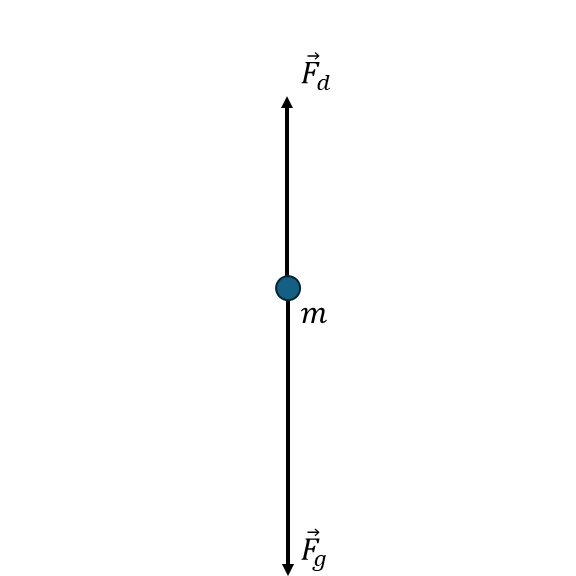
\includegraphics[width=0.98\linewidth]{figs/figure1.png}
%     \caption{Schematic illustation of a free-falling object approaching terminal velocity.}
%     \label{fig:1}
% \end{figure}

% \begin{figure}[H]
%     \centering
%     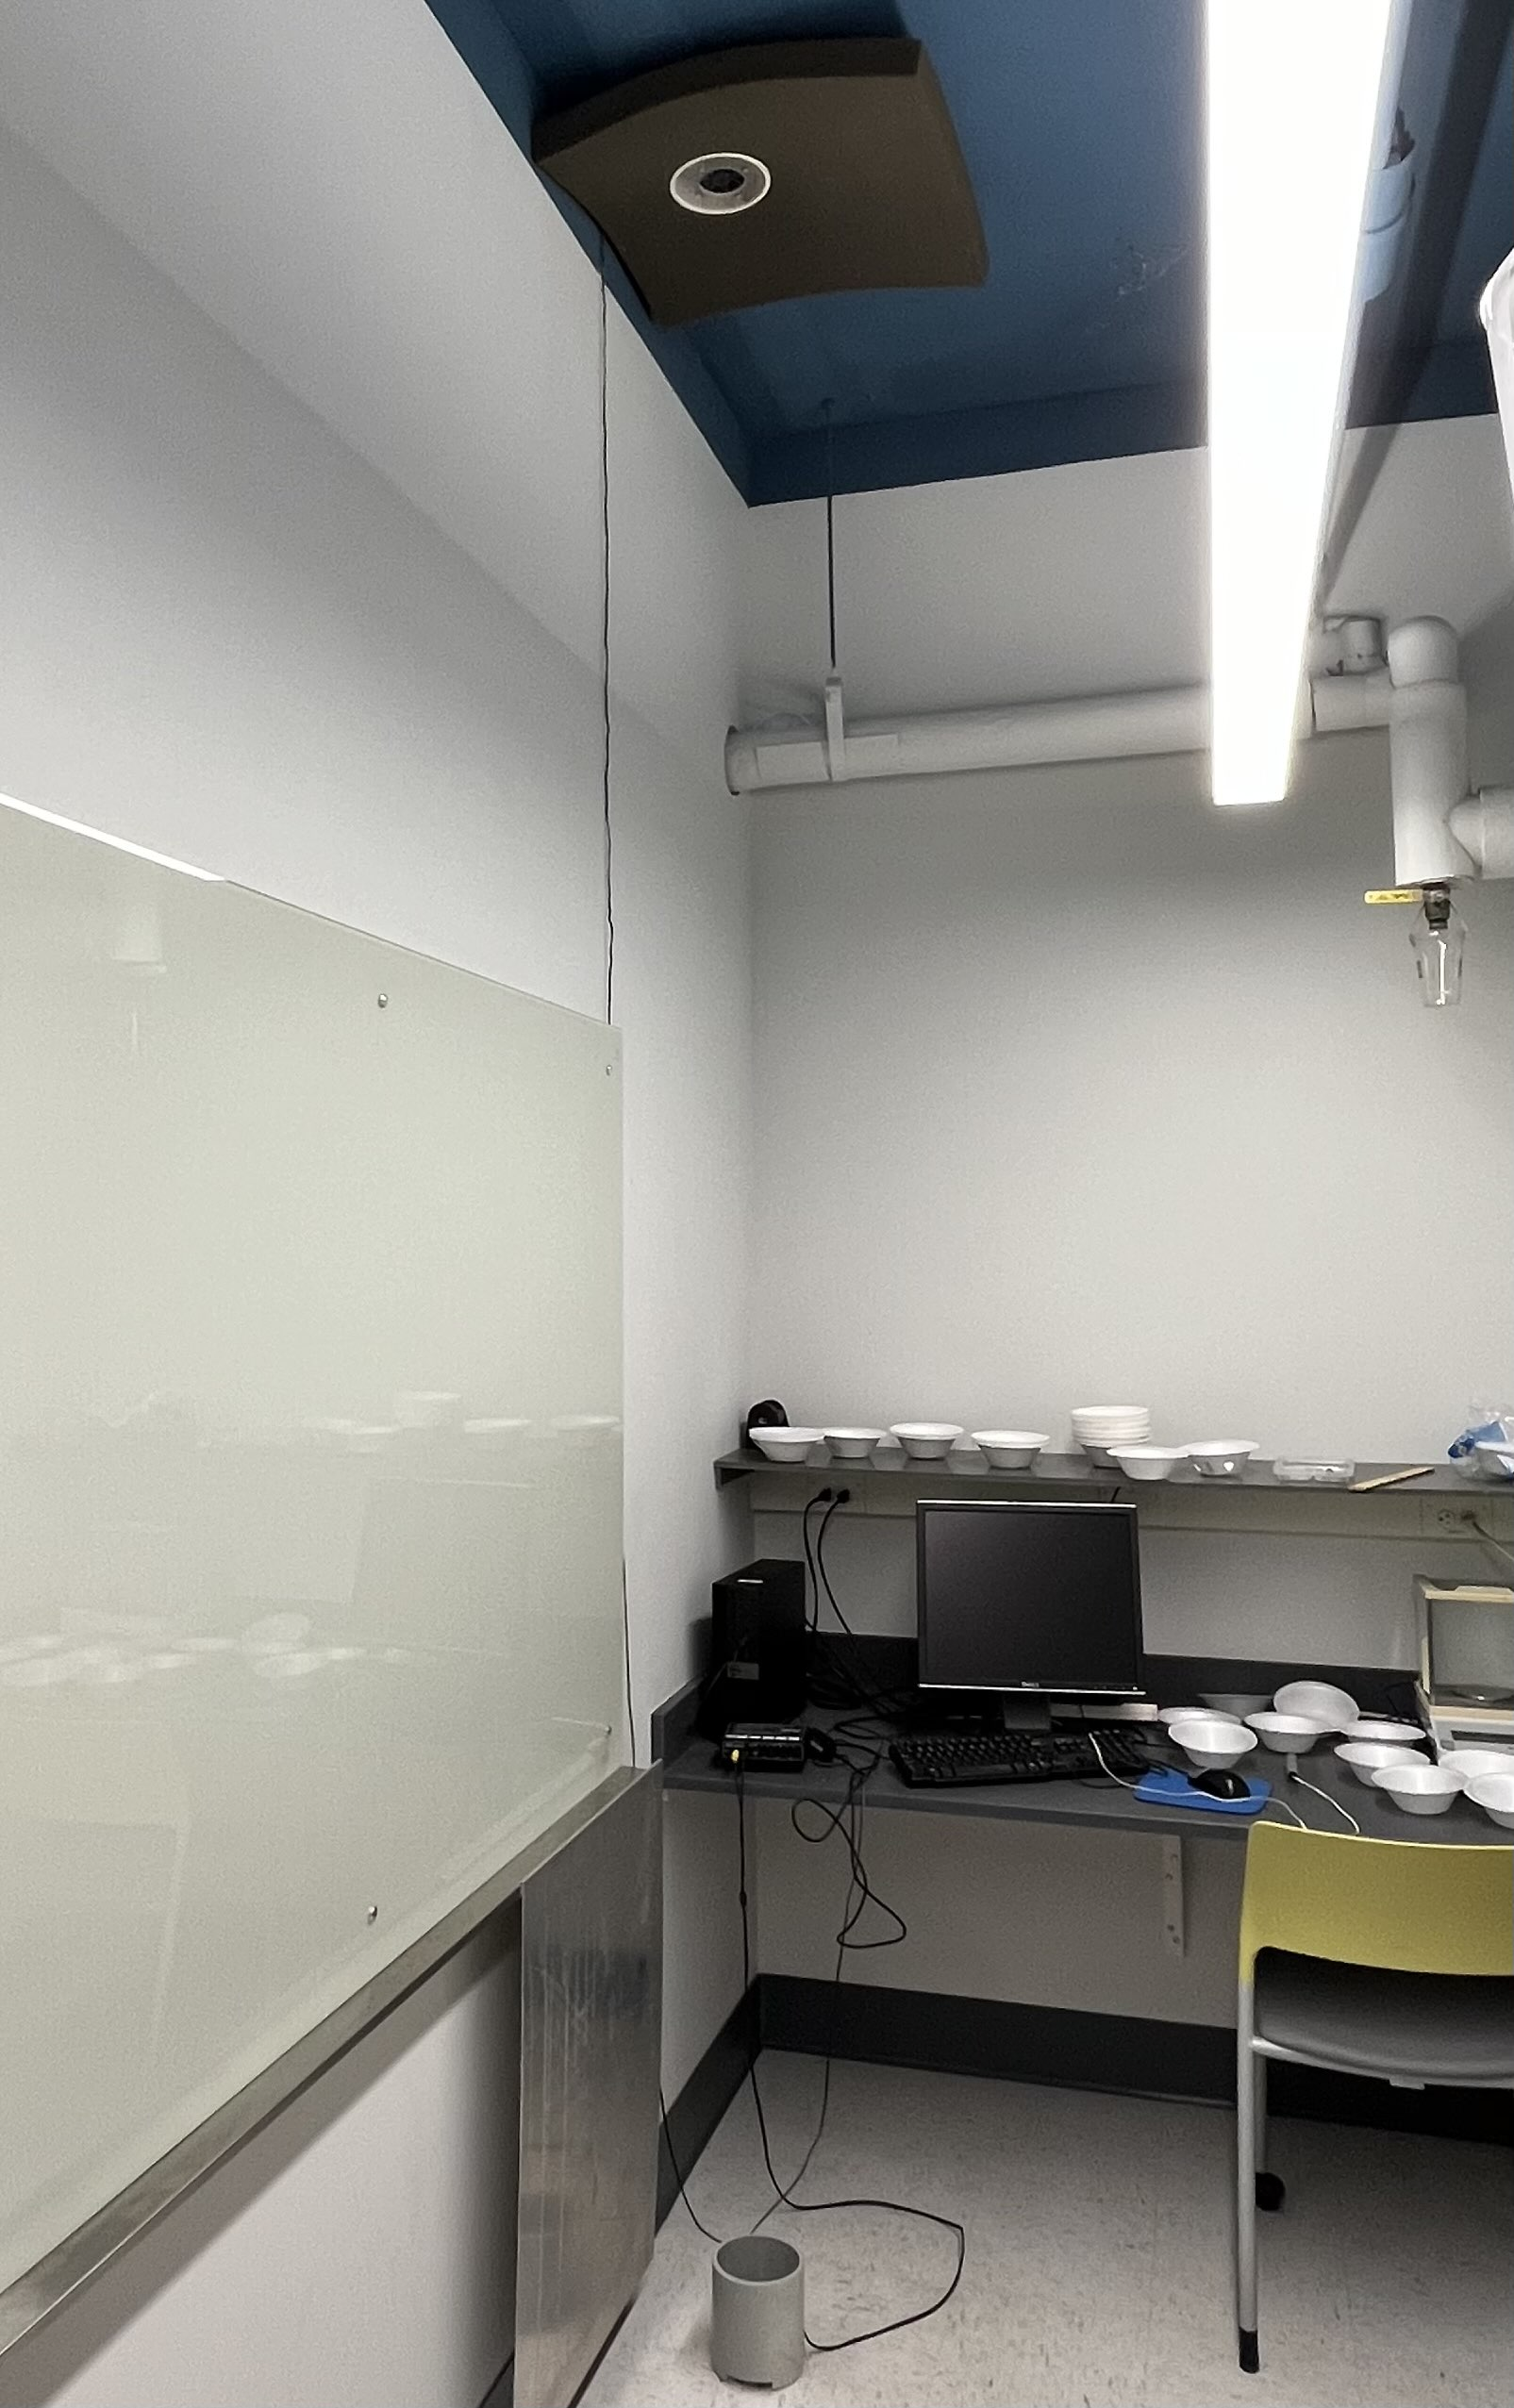
\includegraphics[width=0.98\linewidth]{figs/figure2.jpg}
%     \caption{Photograph of the experimental setup in the lab.}
%     \label{fig:2}
% \end{figure}

% \begin{figure}[H]
%     \centering
%     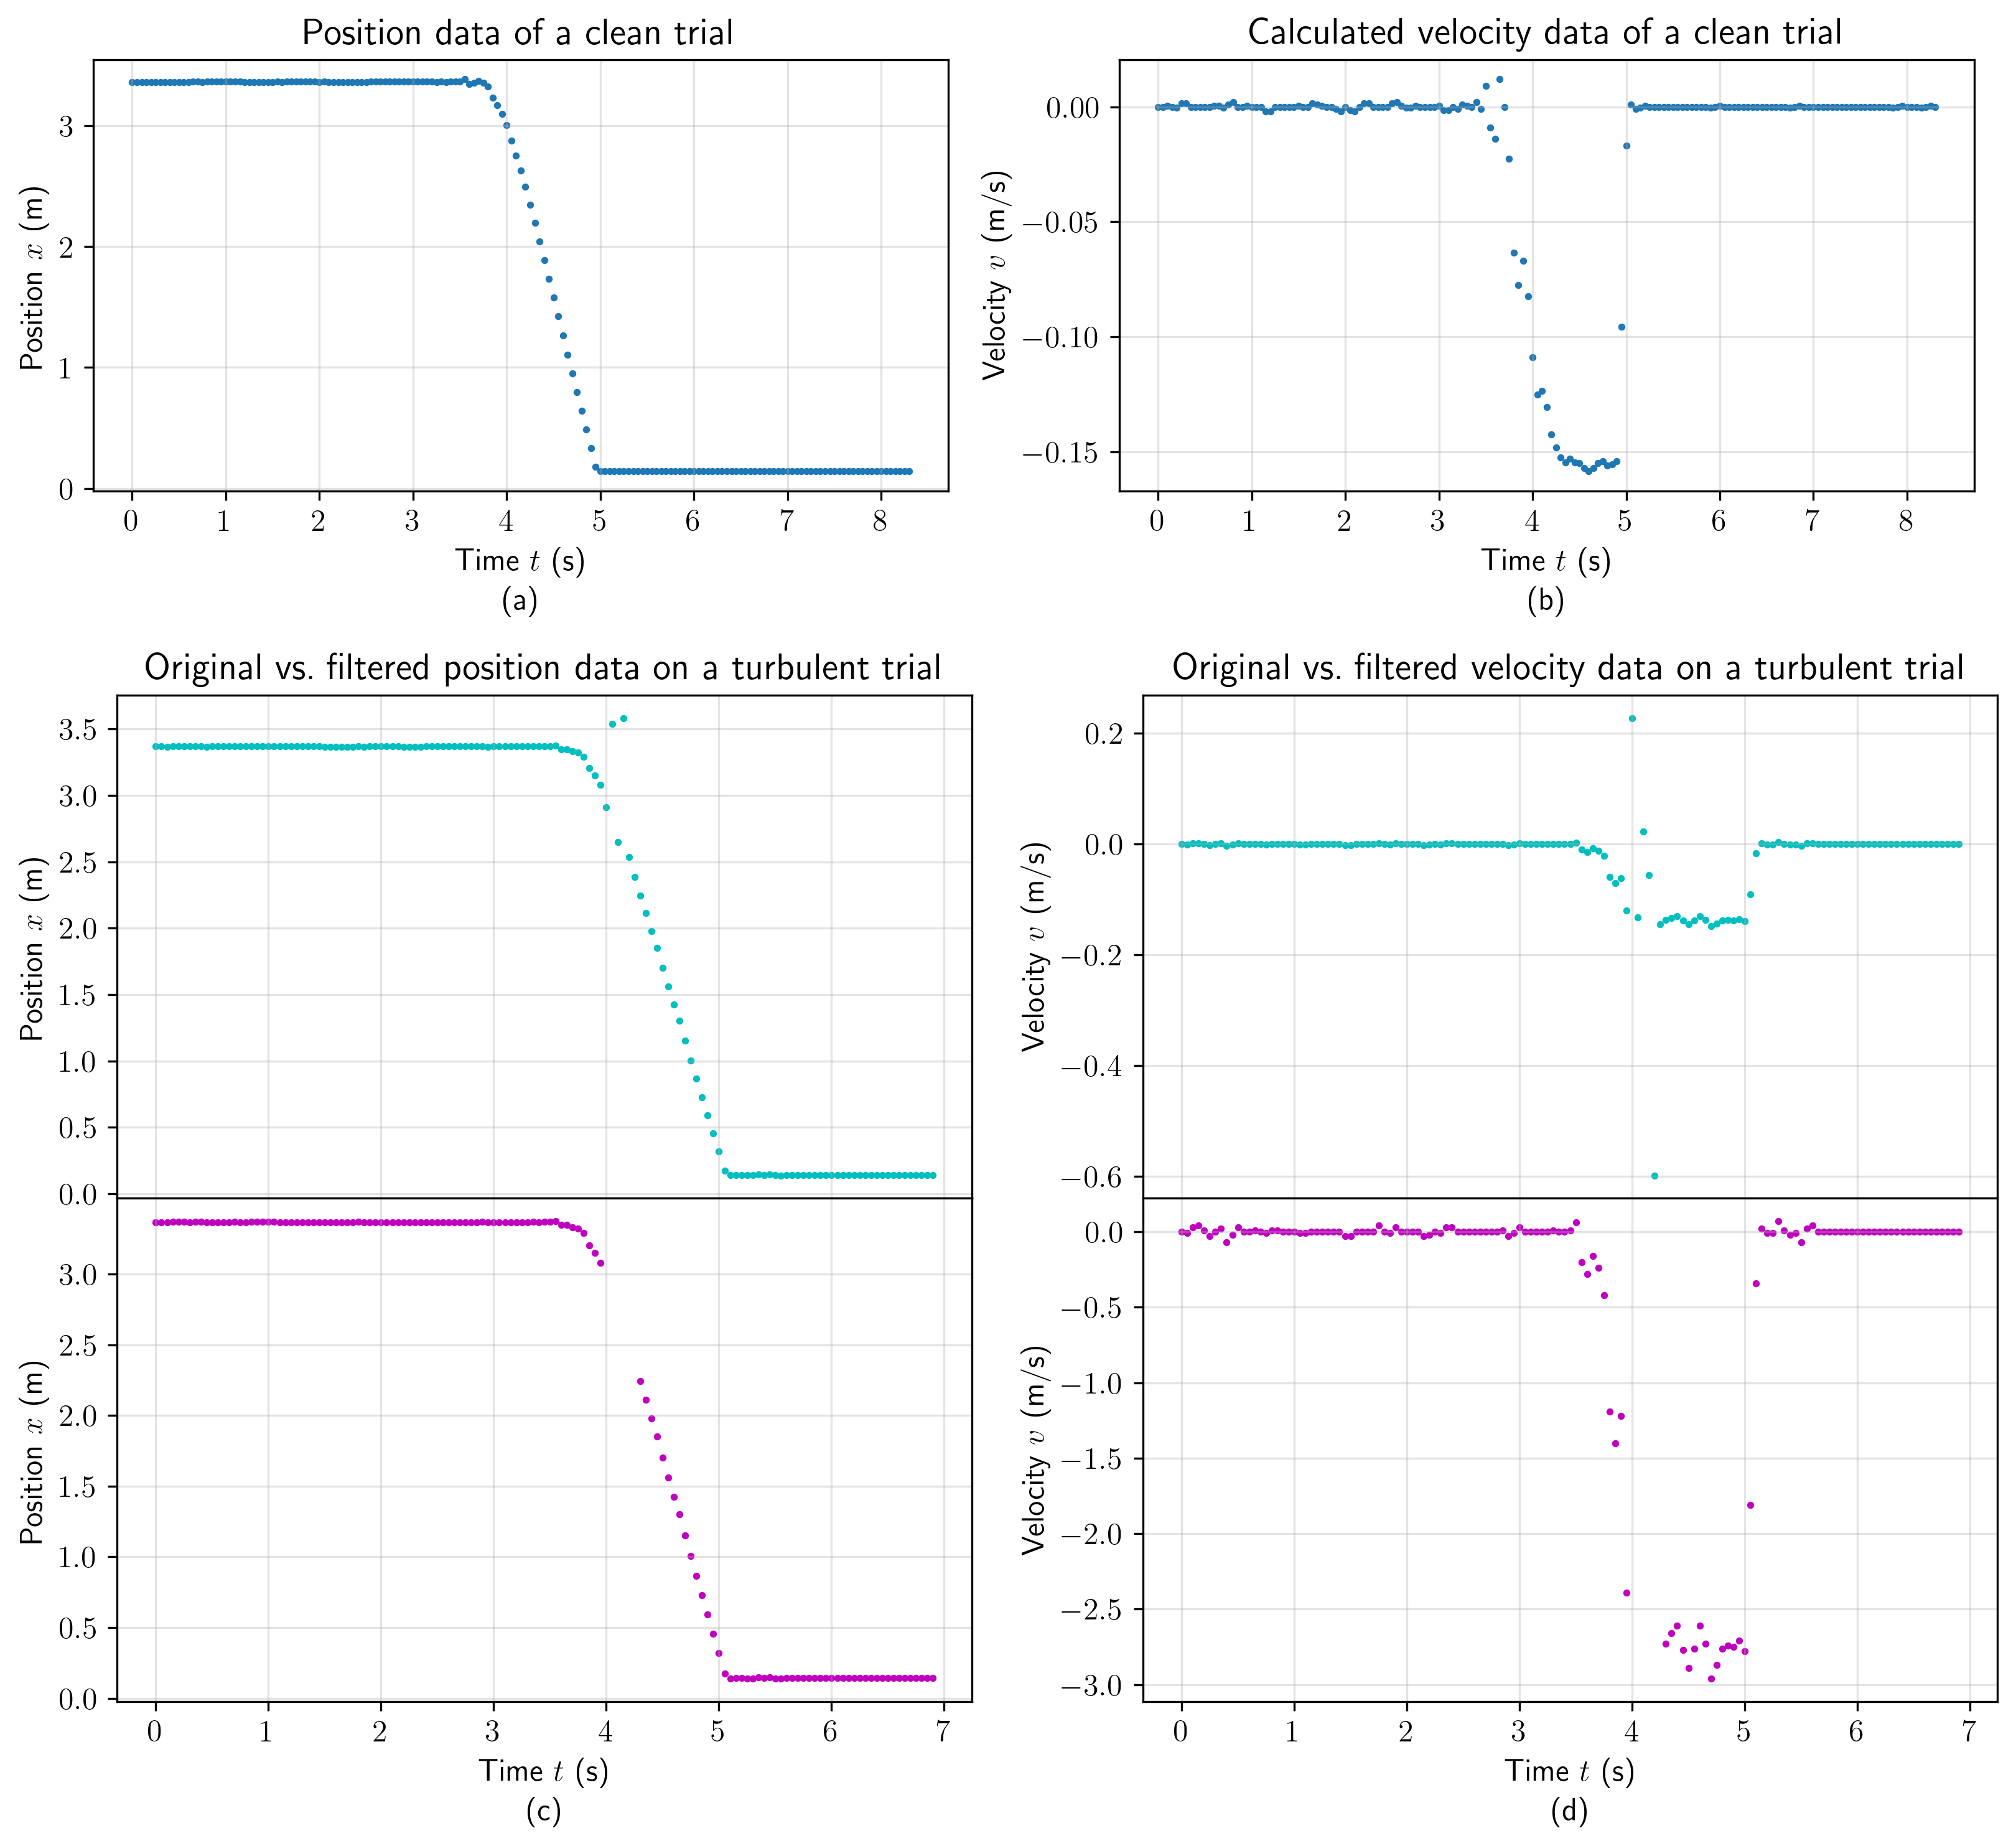
\includegraphics[width=0.98\linewidth]{figs/figure3.png}
%     \caption{
%         Various position vs.\;time and calculated velocity vs.\;time graphs of two sample datasets.
%         (a) \& (b) represents the case of working with a ``clean'' dataset,
%         while (c) \& (d) represents the additional work needed to remove kinks within a turbulent dataset,
%         where the cyan represents the original data from the trial while magenta represents the same data after sufficient filtering.
%         A threshold of 1 for the $Z$-score was used to filter out the outliers for this case.
%     }
%     \label{fig:3}
% \end{figure}

% \begin{figure}[H]
%     \centering
%     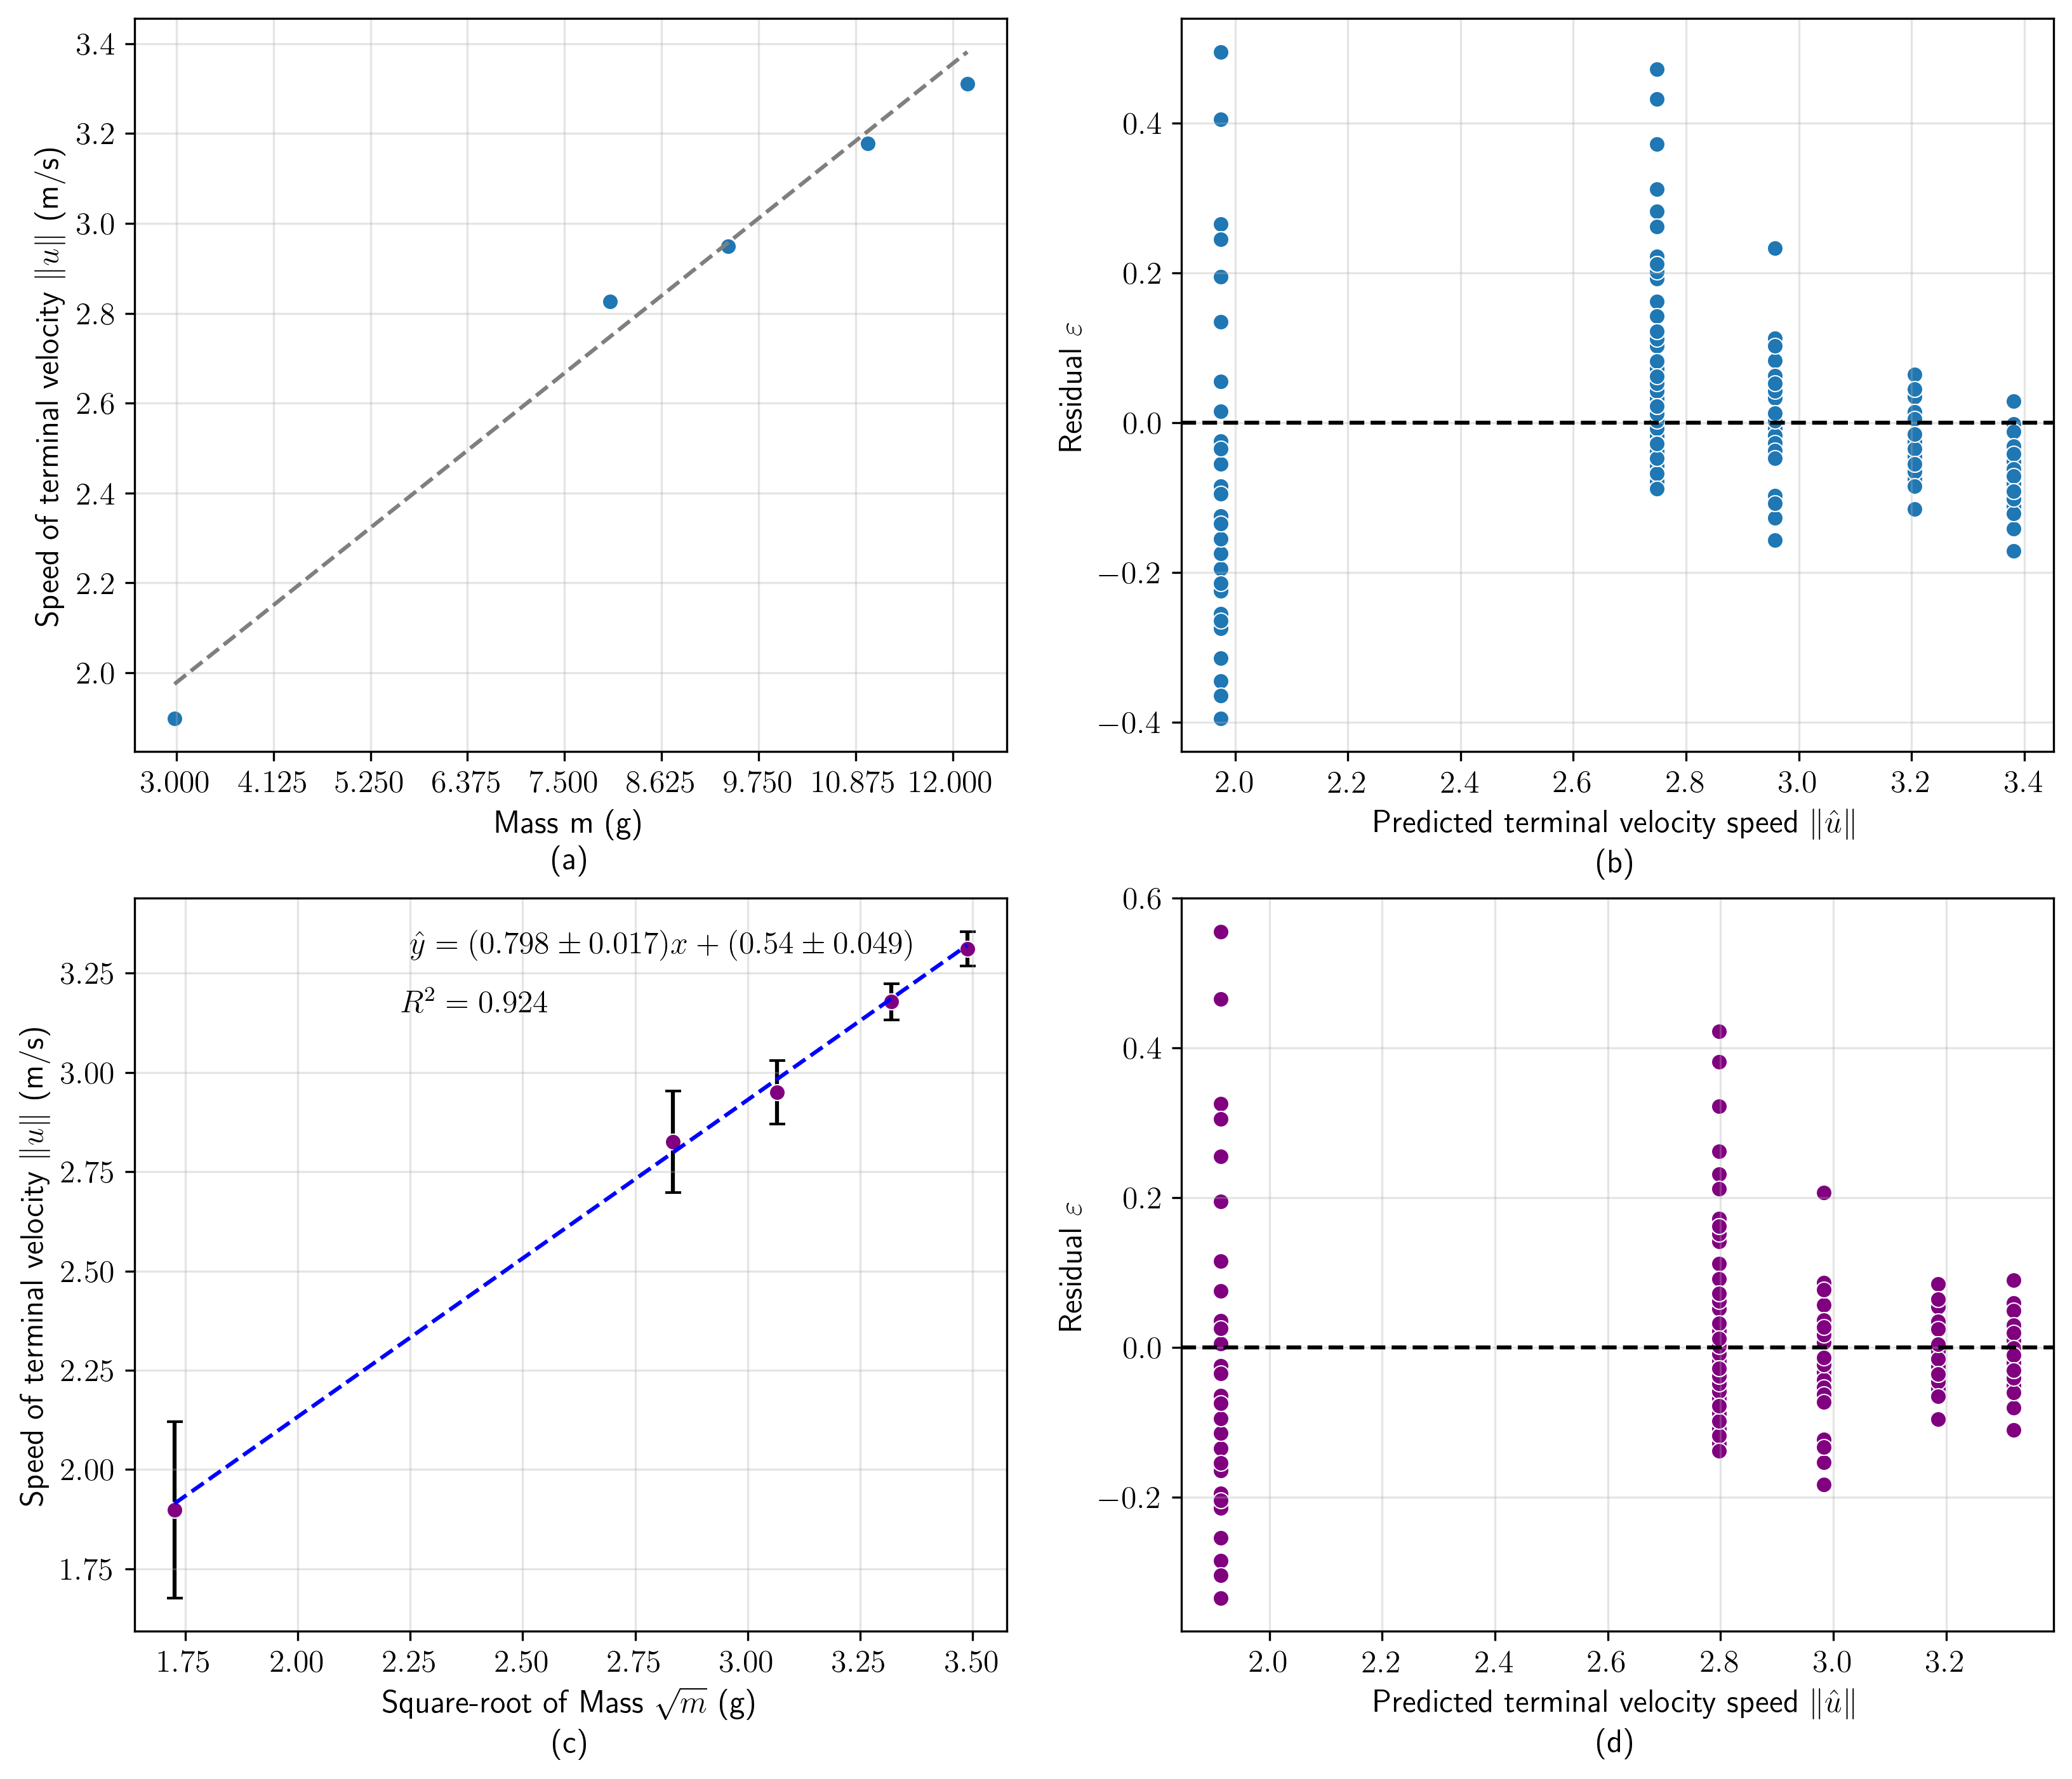
\includegraphics[width=0.98\linewidth]{figs/figure4.png}
%     \caption{
%         Respective linear least-squares fitting for the case when $m$ is untransformed and when it is $\sqrt{m}$.
%         The predictive parameters and $R^2$ value for (a), for it is not included in graph,
%         was found to be $m=0.1530\pm0.004$, $b=1.5191\pm0.032$, and 0.907, respectively,
%         where $\pm$ values represents uncertainties reported in the form of standard deviation.
%         Error bars represent standard deviation in dependent values as uncertainties.
%     }
%     \label{fig:4}
% \end{figure}

% \begin{figure}[H]
%     \centering
%     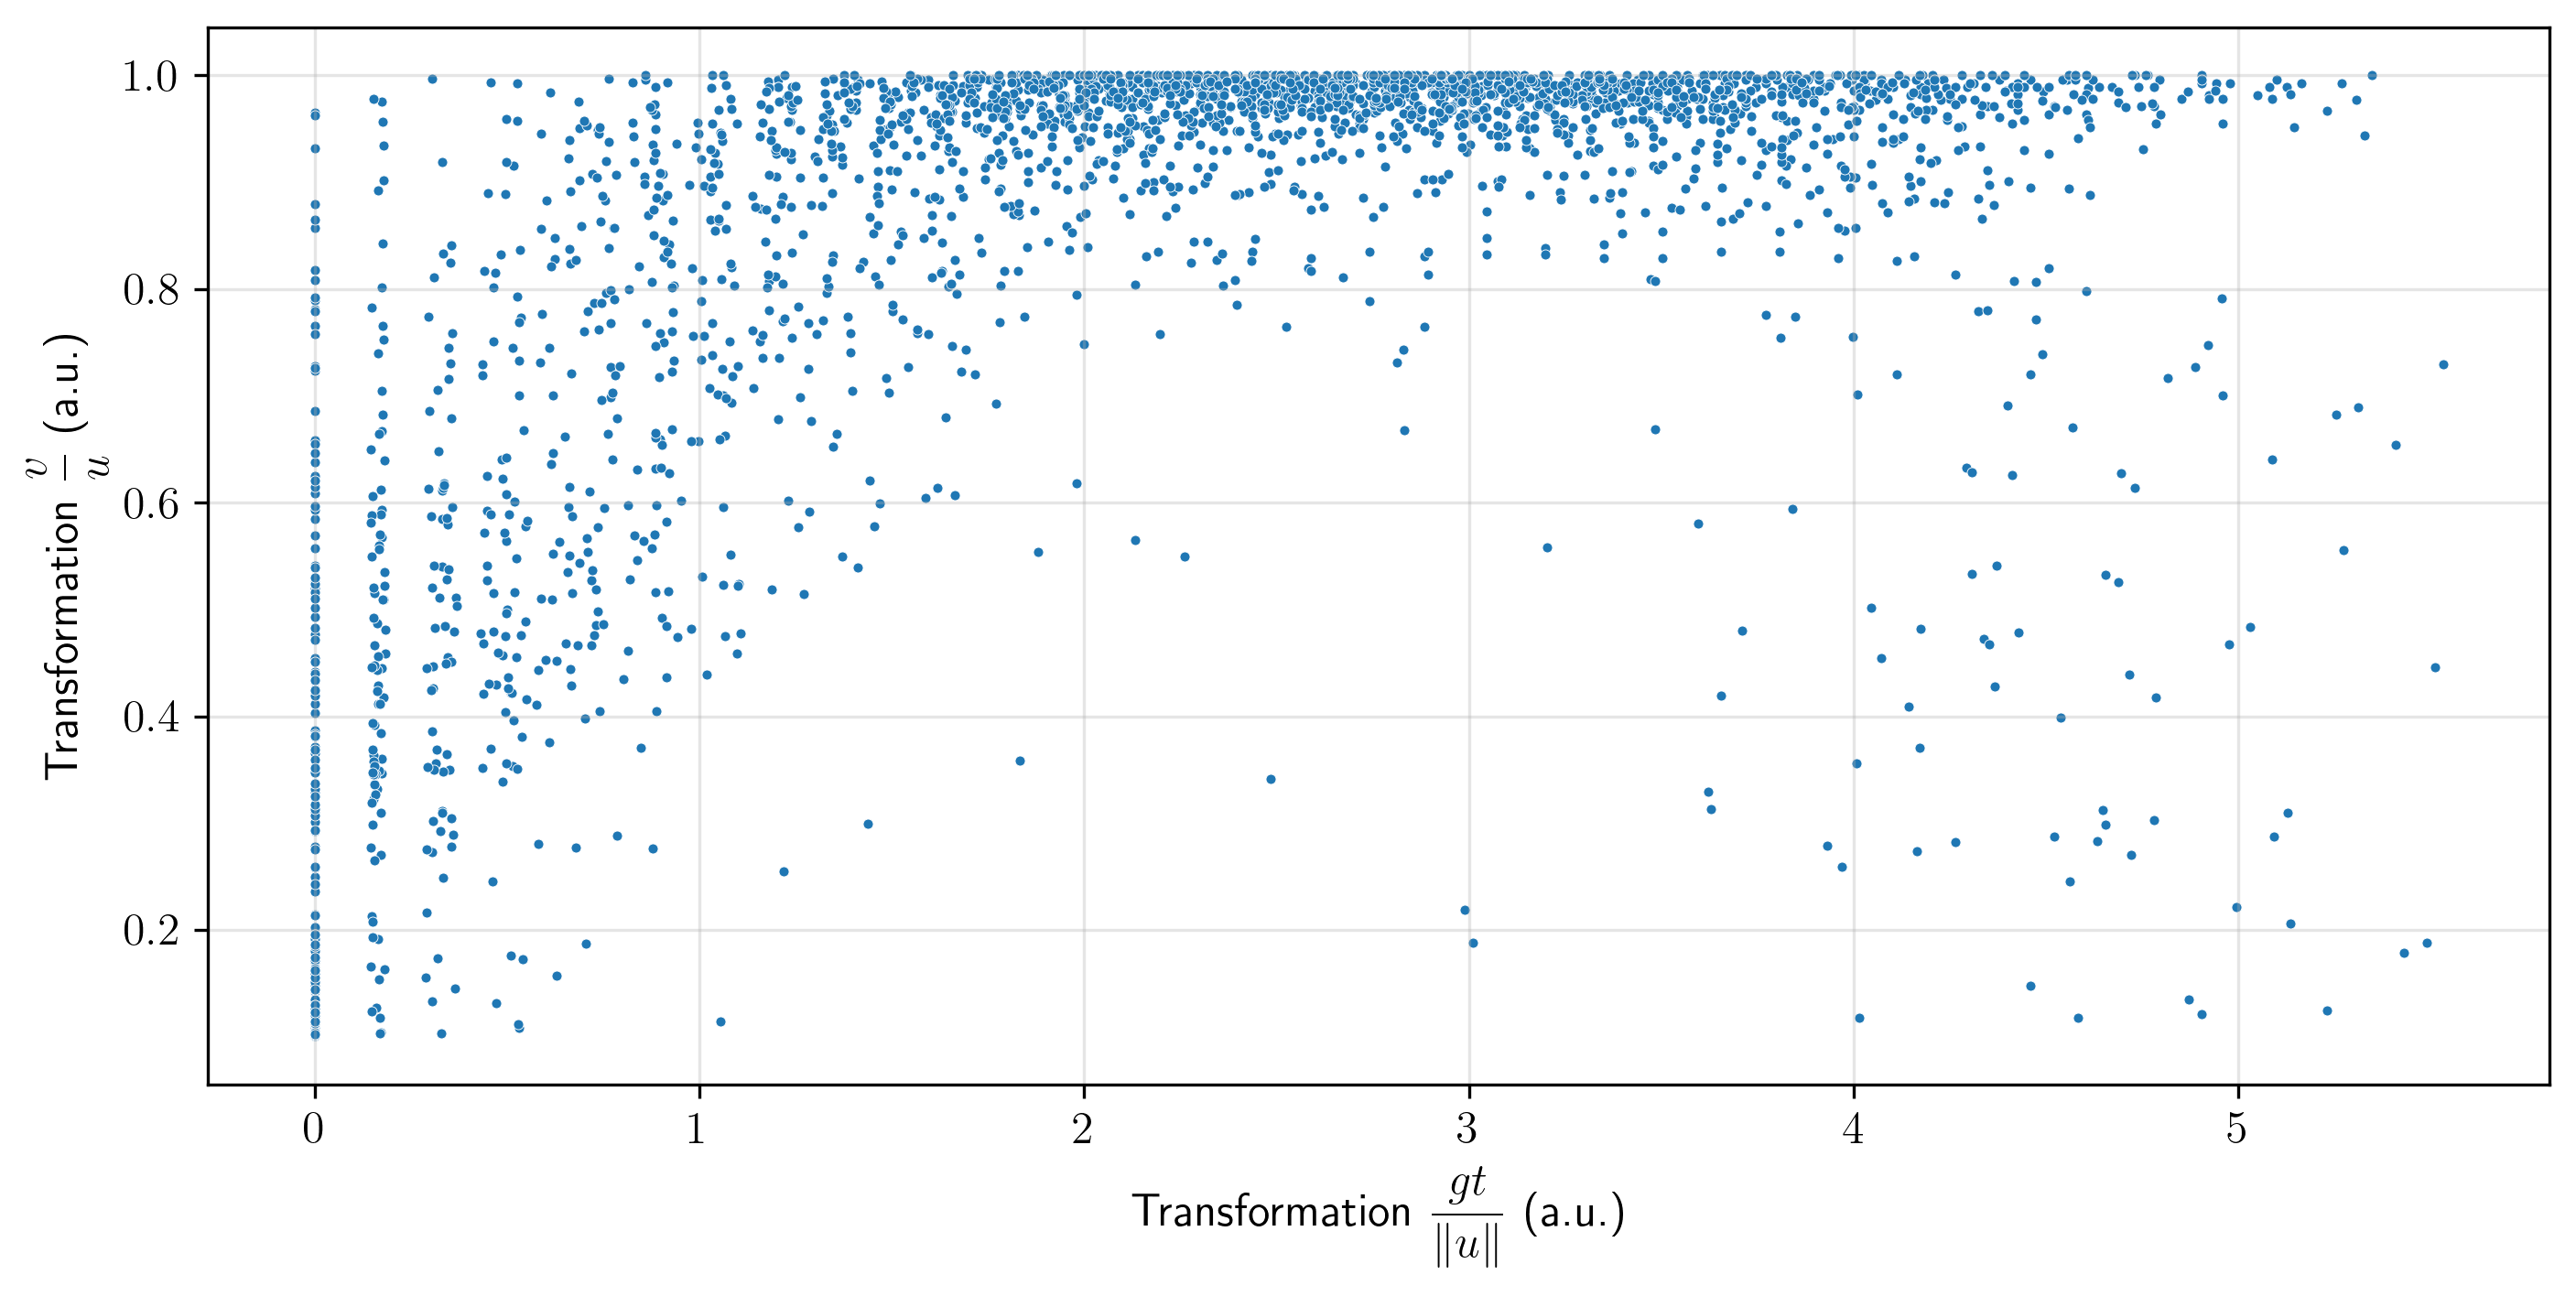
\includegraphics[width=0.98\linewidth]{figs/figure5.png}
%     \caption{
%         Plot of all transformed velocity data gathered across the trials ran for styrofoam bowls 8.029g, 9.397g, 11.1017g, and 12.169g.
%         Datasets were first filtered with a threshold value of 1, transformed as outlined in section \textit{Setup for $y=\tanh(x)$},
%         then further filtered to keep the data values where $0.1\leq\dfrac{v}{u}\leq1$. 
%         Before conglomerating, each trial data had their $x$ data shifted to 0 using the first valid value filtered.
%         Total size of the dataset collection yielded 2760 values.
%     }
%     \label{fig:5}
% \end{figure}

% \begin{figure}
%     \centering
%     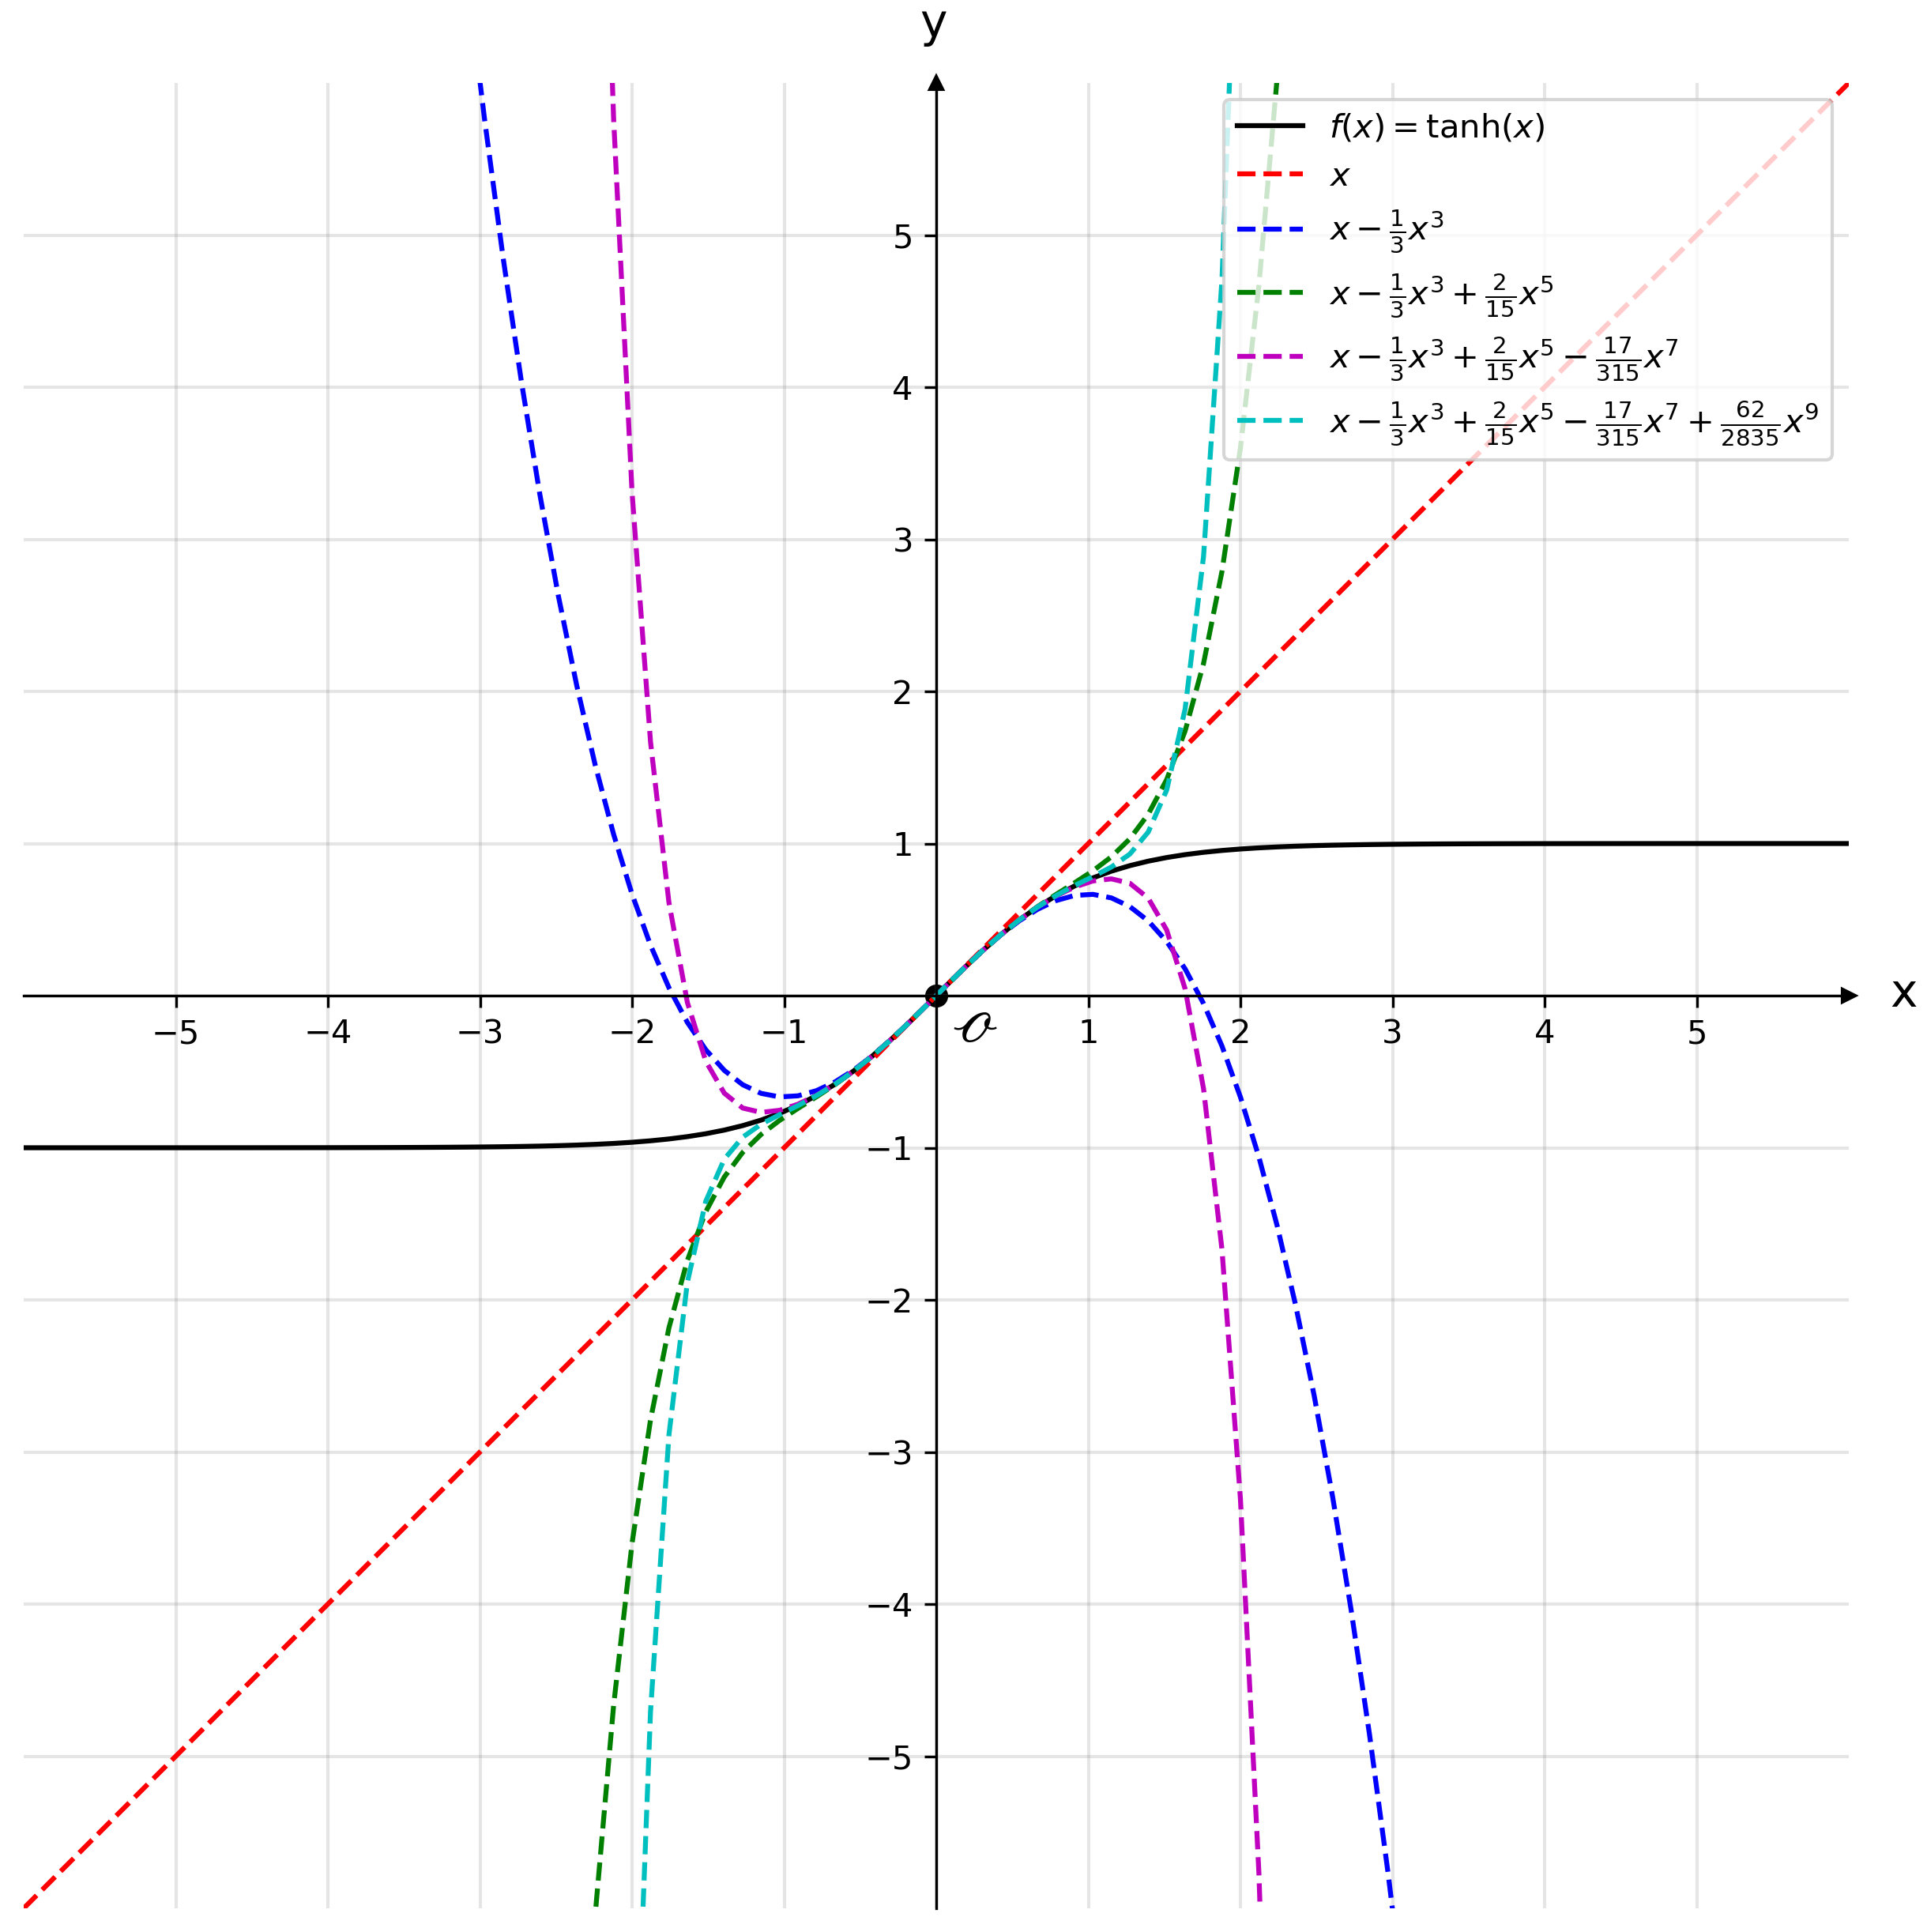
\includegraphics[width=0.98\linewidth]{figs/figure6.png}
%     \caption{
%         Taylor series expansion of $\tanh()$ at $x=0$ up to the 9th order. [\hyperref[sec:5]{5}]
%     }
%     \label{fig:6}
% \end{figure}

% \begin{figure}
%     \centering
%     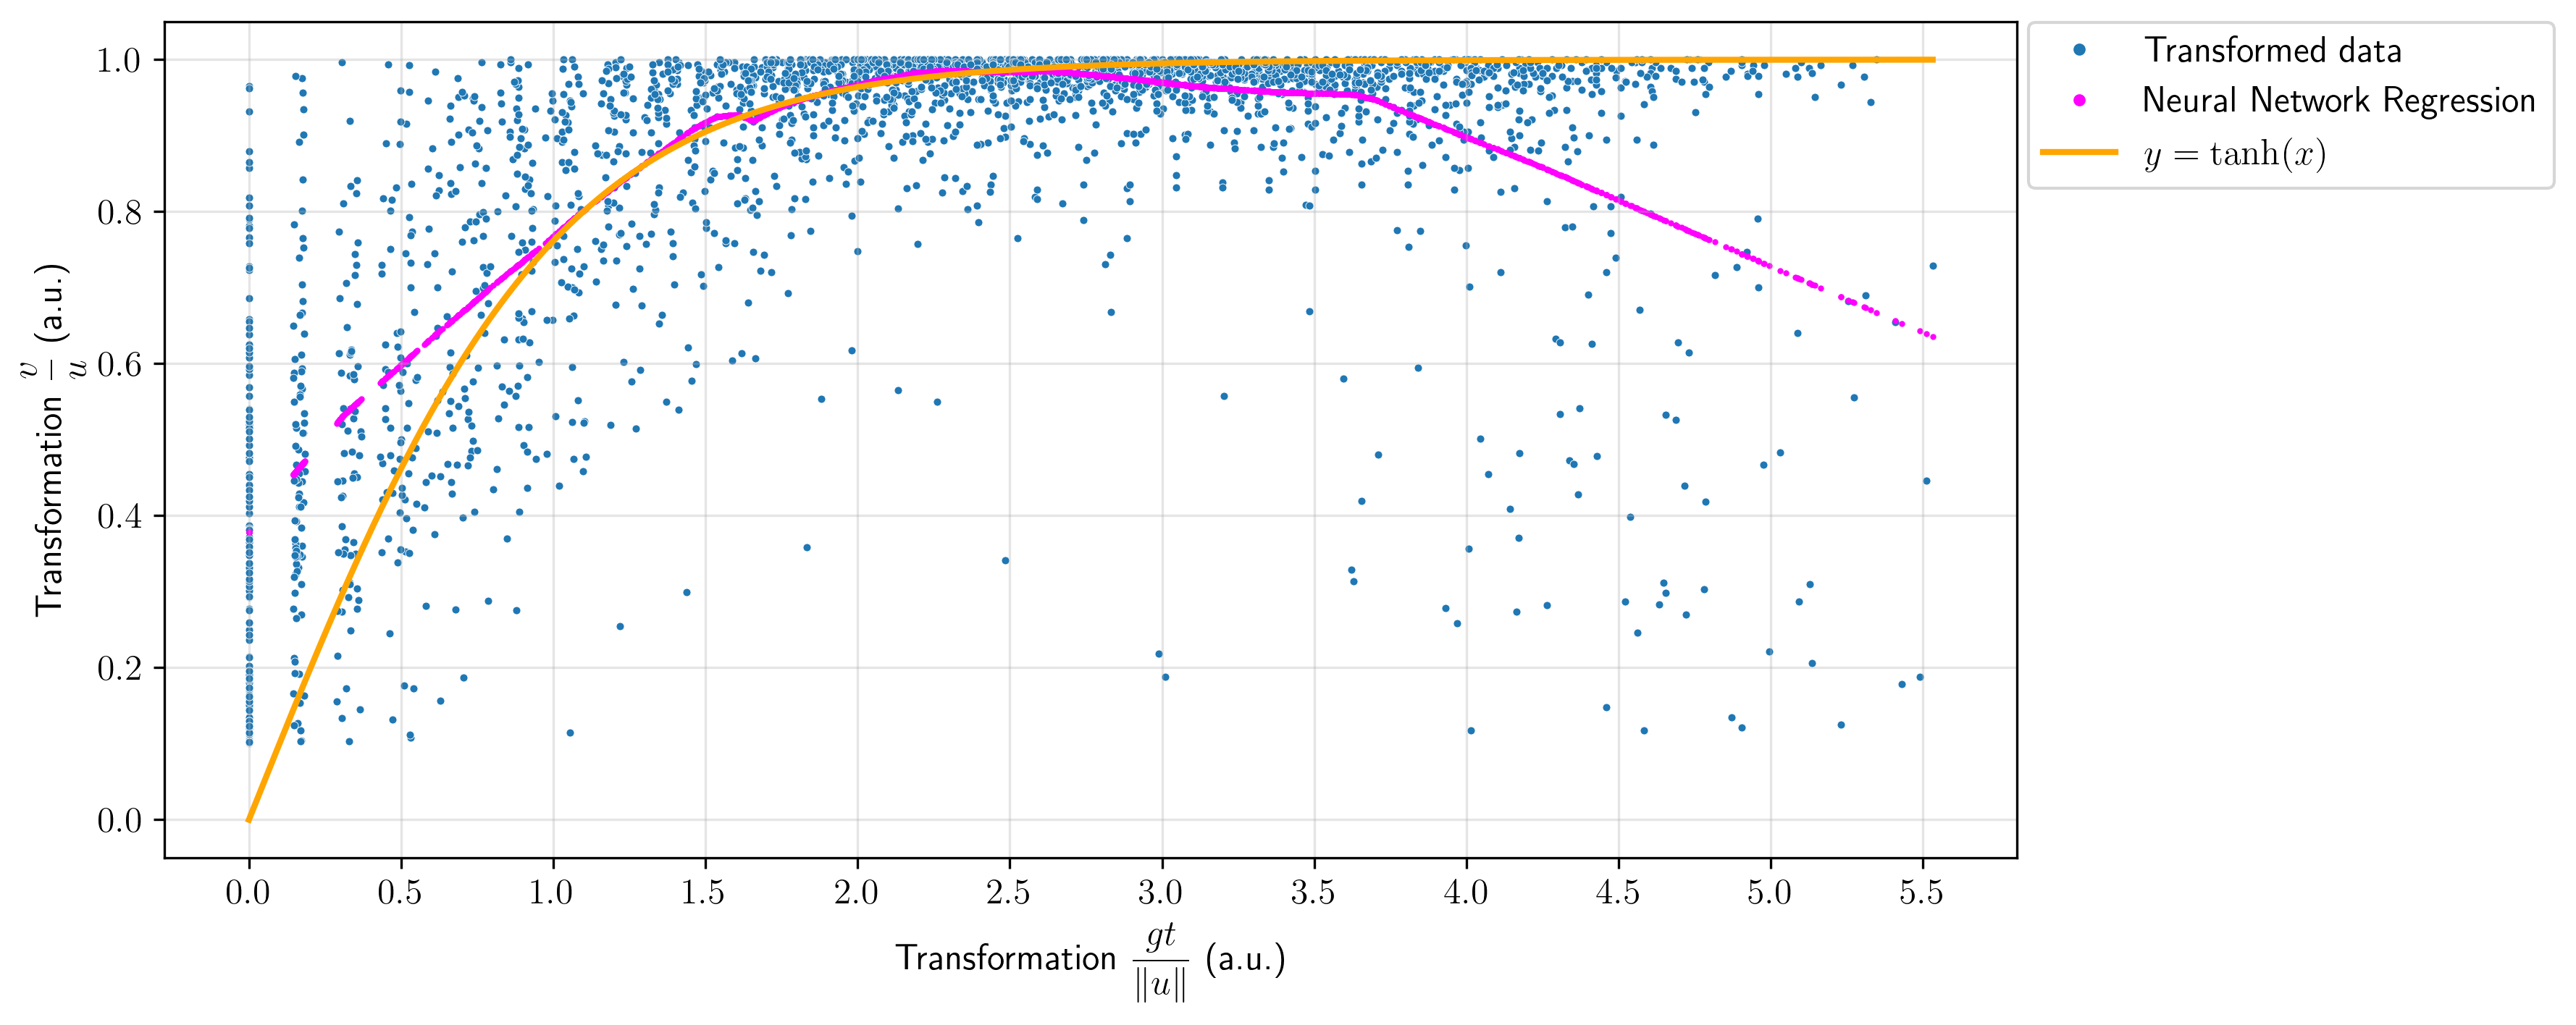
\includegraphics[width=0.98\linewidth]{figs/figure7.png}
%     \caption{
%         Results of the neural network regression on the total transformed velocity dataset.
%         The underlying function, $y=\tanh(x)$, is also plotted for comparison.
%     }
%     \label{fig:7}
% \end{figure}

% \end{multicols}

\end{document}